
%% bare_jrnl.tex
%% V1.4a
%% 2014/09/17
%% by Michael Shell
%% see http://www.michaelshell.org/
%% for current contact information.
%%
%% This is a skeleton file demonstrating the use of IEEEtran.cls
%% (requires IEEEtran.cls version 1.8a or later) with an IEEE
%% journal paper.
%%
%% Support sites:
%% http://www.michaelshell.org/tex/ieeetran/
%% http://www.ctan.org/tex-archive/macros/latex/contrib/IEEEtran/
%% and
%% http://www.ieee.org/

%%*************************************************************************
%% Legal Notice:
%% This code is offered as-is without any warranty either expressed or
%% implied; without even the implied warranty of MERCHANTABILITY or
%% FITNESS FOR A PARTICULAR PURPOSE! 
%% User assumes all risk.
%% In no event shall IEEE or any contributor to this code be liable for
%% any damages or losses, including, but not limited to, incidental,
%% consequential, or any other damages, resulting from the use or misuse
%% of any information contained here.
%%
%% All comments are the opinions of their respective authors and are not
%% necessarily endorsed by the IEEE.
%%
%% This work is distributed under the LaTeX Project Public License (LPPL)
%% ( http://www.latex-project.org/ ) version 1.3, and may be freely used,
%% distributed and modified. A copy of the LPPL, version 1.3, is included
%% in the base LaTeX documentation of all distributions of LaTeX released
%% 2003/12/01 or later.
%% Retain all contribution notices and credits.
%% ** Modified files should be clearly indicated as such, including  **
%% ** renaming them and changing author support contact information. **
%%
%% File list of work: IEEEtran.cls, IEEEtran_HOWTO.pdf, bare_adv.tex,
%%                    bare_conf.tex, bare_jrnl.tex, bare_conf_compsoc.tex,
%%                    bare_jrnl_compsoc.tex, bare_jrnl_transmag.tex
%%*************************************************************************


% *** Authors should verify (and, if needed, correct) their LaTeX system  ***
% *** with the testflow diagnostic prior to trusting their LaTeX platform ***
% *** with production work. IEEE's font choices and paper sizes can       ***
% *** trigger bugs that do not appear when using other class files.       ***                          ***
% The testflow support page is at:
% http://www.michaelshell.org/tex/testflow/



%\documentclass[journal]{IEEEtran}
\documentclass[12pt, draftclsnofoot, onecolumn]{IEEEtran}
%\documentclass[12pt,paper,final]{article}
%
%\documentclass[12pt, onecolummn]{report}
% If IEEEtran.cls has not been installed into the LaTeX system files,
% manually specify the path to it like:
% \documentclass[journal]{../sty/IEEEtran}

\usepackage[latin1]{inputenc}
\usepackage{amsfonts}
\usepackage{amssymb}
\usepackage{amsthm}
\usepackage{fullpage}
\usepackage{setspace}
\usepackage{graphicx}
%\usepackage[pdftex]{graphicx}
\usepackage{psfrag}
\usepackage{color}
\usepackage{epsfig}
%\usepackage{appendix}
%\usepackage{caption}
\usepackage{cite}
\usepackage{ifpdf}
\usepackage[cmex10]{amsmath}
\usepackage{algorithm}
\usepackage{array}
\usepackage{stfloats}
\usepackage{url}
\usepackage{fixltx2e}
\usepackage{setspace} 
\usepackage{diagbox}
\usepackage{subfigure}
\usepackage{algpseudocode}


% Some very useful LaTeX packages include:
% (uncomment the ones you want to load)


% *** MISC UTILITY PACKAGES ***
%
\usepackage{ifpdf}
% Heiko Oberdiek's ifpdf.sty is very useful if you need conditional
% compilation based on whether the output is pdf or dvi.
% usage:
% \ifpdf
%   % pdf code
% \else
%   % dvi code
% \fi
% The latest version of ifpdf.sty can be obtained from:
% http://www.ctan.org/tex-archive/macros/latex/contrib/oberdiek/
% Also, note that IEEEtran.cls V1.7 and later provides a builtin
% \ifCLASSINFOpdf conditional that works the same way.
% When switching from latex to pdflatex and vice-versa, the compiler may
% have to be run twice to clear warning/error messages.






% *** CITATION PACKAGES ***
%
\usepackage{cite}
% cite.sty was written by Donald Arseneau
% V1.6 and later of IEEEtran pre-defines the format of the cite.sty package
% \cite{} output to follow that of IEEE. Loading the cite package will
% result in citation numbers being automatically sorted and properly
% "compressed/ranged". e.g., [1], [9], [2], [7], [5], [6] without using
% cite.sty will become [1], [2], [5]--[7], [9] using cite.sty. cite.sty's
% \cite will automatically add leading space, if needed. Use cite.sty's
% noadjust option (cite.sty V3.8 and later) if you want to turn this off
% such as if a citation ever needs to be enclosed in parenthesis.
% cite.sty is already installed on most LaTeX systems. Be sure and use
% version 5.0 (2009-03-20) and later if using hyperref.sty.
% The latest version can be obtained at:
% http://www.ctan.org/tex-archive/macros/latex/contrib/cite/
% The documentation is contained in the cite.sty file itself.






% *** GRAPHICS RELATED PACKAGES ***
%
\ifCLASSINFOpdf
  % \usepackage[pdftex]{graphicx}
  % declare the path(s) where your graphic files are
  % \graphicspath{{../pdf/}{../jpeg/}}
  % and their extensions so you won't have to specify these with
  % every instance of \includegraphics
  % \DeclareGraphicsExtensions{.pdf,.jpeg,.png}
\else
  % or other class option (dvipsone, dvipdf, if not using dvips). graphicx
  % will default to the driver specified in the system graphics.cfg if no
  % driver is specified.
  % \usepackage[dvips]{graphicx}
  % declare the path(s) where your graphic files are
  % \graphicspath{{../eps/}}
  % and their extensions so you won't have to specify these with
  % every instance of \includegraphics
  % \DeclareGraphicsExtensions{.eps}
\fi
% graphicx was written by David Carlisle and Sebastian Rahtz. It is
% required if you want graphics, photos, etc. graphicx.sty is already
% installed on most LaTeX systems. The latest version and documentation
% can be obtained at: 
% http://www.ctan.org/tex-archive/macros/latex/required/graphics/
% Another good source of documentation is "Using Imported Graphics in
% LaTeX2e" by Keith Reckdahl which can be found at:
% http://www.ctan.org/tex-archive/info/epslatex/
%
% latex, and pdflatex in dvi mode, support graphics in encapsulated
% postscript (.eps) format. pdflatex in pdf mode supports graphics
% in .pdf, .jpeg, .png and .mps (metapost) formats. Users should ensure
% that all non-photo figures use a vector format (.eps, .pdf, .mps) and
% not a bitmapped formats (.jpeg, .png). IEEE frowns on bitmapped formats
% which can result in "jaggedy"/blurry rendering of lines and letters as
% well as large increases in file sizes.
%
% You can find documentation about the pdfTeX application at:
% http://www.tug.org/applications/pdftex





% *** MATH PACKAGES ***
%
\usepackage[cmex10]{amsmath}
% A popular package from the American Mathematical Society that provides
% many useful and powerful commands for dealing with mathematics. If using
% it, be sure to load this package with the cmex10 option to ensure that
% only type 1 fonts will utilized at all point sizes. Without this option,
% it is possible that some math symbols, particularly those within
% footnotes, will be rendered in bitmap form which will result in a
% document that can not be IEEE Xplore compliant!
%
% Also, note that the amsmath package sets \interdisplaylinepenalty to 10000
% thus preventing page breaks from occurring within multiline equations. Use:
%\interdisplaylinepenalty=2500
% after loading amsmath to restore such page breaks as IEEEtran.cls normally
% does. amsmath.sty is already installed on most LaTeX systems. The latest
% version and documentation can be obtained at:
% http://www.ctan.org/tex-archive/macros/latex/required/amslatex/math/





% *** SPECIALIZED LIST PACKAGES ***
%
%\usepackage{algorithmic}
% algorithmic.sty was written by Peter Williams and Rogerio Brito.
% This package provides an algorithmic environment fo describing algorithms.
% You can use the algorithmic environment in-text or within a figure
% environment to provide for a floating algorithm. Do NOT use the algorithm
% floating environment provided by algorithm.sty (by the same authors) or
% algorithm2e.sty (by Christophe Fiorio) as IEEE does not use dedicated
% algorithm float types and packages that provide these will not provide
% correct IEEE style captions. The latest version and documentation of
% algorithmic.sty can be obtained at:
% http://www.ctan.org/tex-archive/macros/latex/contrib/algorithms/
% There is also a support site at:
% http://algorithms.berlios.de/index.html
% Also of interest may be the (relatively newer and more customizable)
% algorithmicx.sty package by Szasz Janos:
% http://www.ctan.org/tex-archive/macros/latex/contrib/algorithmicx/




% *** ALIGNMENT PACKAGES ***
%
\usepackage{array}
% Frank Mittelbach's and David Carlisle's array.sty patches and improves
% the standard LaTeX2e array and tabular environments to provide better
% appearance and additional user controls. As the default LaTeX2e table
% generation code is lacking to the point of almost being broken with
% respect to the quality of the end results, all users are strongly
% advised to use an enhanced (at the very least that provided by array.sty)
% set of table tools. array.sty is already installed on most systems. The
% latest version and documentation can be obtained at:
% http://www.ctan.org/tex-archive/macros/latex/required/tools/


% IEEEtran contains the IEEEeqnarray family of commands that can be used to
% generate multiline equations as well as matrices, tables, etc., of high
% quality.




% *** SUBFIGURE PACKAGES ***
%\ifCLASSOPTIONcompsoc
%  \usepackage[caption=false,font=normalsize,labelfont=sf,textfont=sf]{subfig}
%\else
%  \usepackage[caption=false,font=footnotesize]{subfig}
%\fi
% subfig.sty, written by Steven Douglas Cochran, is the modern replacement
% for subfigure.sty, the latter of which is no longer maintained and is
% incompatible with some LaTeX packages including fixltx2e. However,
% subfig.sty requires and automatically loads Axel Sommerfeldt's caption.sty
% which will override IEEEtran.cls' handling of captions and this will result
% in non-IEEE style figure/table captions. To prevent this problem, be sure
% and invoke subfig.sty's "caption=false" package option (available since
% subfig.sty version 1.3, 2005/06/28) as this is will preserve IEEEtran.cls
% handling of captions.
% Note that the Computer Society format requires a larger sans serif font
% than the serif footnote size font used in traditional IEEE formatting
% and thus the need to invoke different subfig.sty package options depending
% on whether compsoc mode has been enabled.
%
% The latest version and documentation of subfig.sty can be obtained at:
% http://www.ctan.org/tex-archive/macros/latex/contrib/subfig/




% *** FLOAT PACKAGES ***
%
\usepackage{fixltx2e}
% fixltx2e, the successor to the earlier fix2col.sty, was written by
% Frank Mittelbach and David Carlisle. This package corrects a few problems
% in the LaTeX2e kernel, the most notable of which is that in current
% LaTeX2e releases, the ordering of single and double column floats is not
% guaranteed to be preserved. Thus, an unpatched LaTeX2e can allow a
% single column figure to be placed prior to an earlier double column
% figure. The latest version and documentation can be found at:
% http://www.ctan.org/tex-archive/macros/latex/base/


%\usepackage{stfloats}
% stfloats.sty was written by Sigitas Tolusis. This package gives LaTeX2e
% the ability to do double column floats at the bottom of the page as well
% as the top. (e.g., "\begin{figure*}[!b]" is not normally possible in
% LaTeX2e). It also provides a command:
%\fnbelowfloat
% to enable the placement of footnotes below bottom floats (the standard
% LaTeX2e kernel puts them above bottom floats). This is an invasive package
% which rewrites many portions of the LaTeX2e float routines. It may not work
% with other packages that modify the LaTeX2e float routines. The latest
% version and documentation can be obtained at:
% http://www.ctan.org/tex-archive/macros/latex/contrib/sttools/
% Do not use the stfloats baselinefloat ability as IEEE does not allow
% \baselineskip to stretch. Authors submitting work to the IEEE should note
% that IEEE rarely uses double column equations and that authors should try
% to avoid such use. Do not be tempted to use the cuted.sty or midfloat.sty
% packages (also by Sigitas Tolusis) as IEEE does not format its papers in
% such ways.
% Do not attempt to use stfloats with fixltx2e as they are incompatible.
% Instead, use Morten Hogholm'a dblfloatfix which combines the features
% of both fixltx2e and stfloats:
%
% \usepackage{dblfloatfix}
% The latest version can be found at:
% http://www.ctan.org/tex-archive/macros/latex/contrib/dblfloatfix/




%\ifCLASSOPTIONcaptionsoff
%  \usepackage[nomarkers]{endfloat}
% \let\MYoriglatexcaption\caption
% \renewcommand{\caption}[2][\relax]{\MYoriglatexcaption[#2]{#2}}
%\fi
% endfloat.sty was written by James Darrell McCauley, Jeff Goldberg and 
% Axel Sommerfeldt. This package may be useful when used in conjunction with 
% IEEEtran.cls'  captionsoff option. Some IEEE journals/societies require that
% submissions have lists of figures/tables at the end of the paper and that
% figures/tables without any captions are placed on a page by themselves at
% the end of the document. If needed, the draftcls IEEEtran class option or
% \CLASSINPUTbaselinestretch interface can be used to increase the line
% spacing as well. Be sure and use the nomarkers option of endfloat to
% prevent endfloat from "marking" where the figures would have been placed
% in the text. The two hack lines of code above are a slight modification of
% that suggested by in the endfloat docs (section 8.4.1) to ensure that
% the full captions always appear in the list of figures/tables - even if
% the user used the short optional argument of \caption[]{}.
% IEEE papers do not typically make use of \caption[]'s optional argument,
% so this should not be an issue. A similar trick can be used to disable
% captions of packages such as subfig.sty that lack options to turn off
% the subcaptions:
% For subfig.sty:
% \let\MYorigsubfloat\subfloat
% \renewcommand{\subfloat}[2][\relax]{\MYorigsubfloat[]{#2}}
% However, the above trick will not work if both optional arguments of
% the \subfloat command are used. Furthermore, there needs to be a
% description of each subfigure *somewhere* and endfloat does not add
% subfigure captions to its list of figures. Thus, the best approach is to
% avoid the use of subfigure captions (many IEEE journals avoid them anyway)
% and instead reference/explain all the subfigures within the main caption.
% The latest version of endfloat.sty and its documentation can obtained at:
% http://www.ctan.org/tex-archive/macros/latex/contrib/endfloat/
%
% The IEEEtran \ifCLASSOPTIONcaptionsoff conditional can also be used
% later in the document, say, to conditionally put the References on a 
% page by themselves.




% *** PDF, URL AND HYPERLINK PACKAGES ***
%
\usepackage{url}
% url.sty was written by Donald Arseneau. It provides better support for
% handling and breaking URLs. url.sty is already installed on most LaTeX
% systems. The latest version and documentation can be obtained at:
% http://www.ctan.org/tex-archive/macros/latex/contrib/url/
% Basically, \url{my_url_here}.




% *** Do not adjust lengths that control margins, column widths, etc. ***
% *** Do not use packages that alter fonts (such as pslatex).         ***
% There should be no need to do such things with IEEEtran.cls V1.6 and later.
% (Unless specifically asked to do so by the journal or conference you plan
% to submit to, of course. )


% correct bad hyphenation here
\hyphenation{op-tical net-works semi-conduc-tor}


\begin{document}
\begin{spacing}{2}
%\doublespacing
%
% paper title
% Titles are generally capitalized except for words such as a, an, and, as,
% at, but, by, for, in, nor, of, on, or, the, to and up, which are usually
% not capitalized unless they are the first or last word of the title.
% Linebreaks \\ can be used within to get better formatting as desired.
% Do not put math or special symbols in the title.
\title{Report}

%
%
% author names and IEEE memberships
% note positions of commas and nonbreaking spaces ( ~ ) LaTeX will not break
% a structure at a ~ so this keeps an author's name from being broken across
% two lines.
% use \thanks{} to gain access to the first footnote area
% a separate \thanks must be used for each paragraph as LaTeX2e's \thanks
% was not built to handle multiple paragraphs
%
\author{Tianpei Chen\\
Department of Electrical and Computer Engineering\\
McGill University\\
\today}

%\author{Michael~Shell,~\IEEEmembership{Member,~IEEE,}
%        John~Doe,~\IEEEmembership{Fellow,~OSA,}
%        and~Jane~Doe,~\IEEEmembership{Life~Fellow,~IEEE}% <-this % stops a space
%\thanks{M. Shell is with the Department
%of Electrical and Computer Engineering, Georgia Institute of Technology, Atlanta,
%GA, 30332 USA e-mail: (see http://www.michaelshell.org/contact.html).}% <-this % stops a space
%\thanks{J. Doe and J. Doe are with Anonymous University.}% <-this % stops a space
%\thanks{Manuscript received April 19, 2005; revised September 17, 2014.}}

% note the % following the last \IEEEmembership and also \thanks - 
% these prevent an unwanted space from occurring between the last author name
% and the end of the author line. i.e., if you had this:
% 
% \author{....lastname \thanks{...} \thanks{...} }
%                     ^------------^------------^----Do not want these spaces!
%
% a space would be appended to the last name and could cause every name on that
% line to be shifted left slightly. This is one of those "LaTeX things". For
% instance, "\textbf{A} \textbf{B}" will typeset as "A B" not "AB". To get
% "AB" then you have to do: "\textbf{A}\textbf{B}"
% \thanks is no different in this regard, so shield the last } of each \thanks
% that ends a line with a % and do not let a space in before the next \thanks.
% Spaces after \IEEEmembership other than the last one are OK (and needed) as
% you are supposed to have spaces between the names. For what it is worth,
% this is a minor point as most people would not even notice if the said evil
% space somehow managed to creep in.



% The paper headers
%\markboth{Journal of \LaTeX\ Class Files,~Vol.~13, No.~9, September~2014}%
%{Shell \MakeLowercase{\textit{et al.}}: Bare Demo of IEEEtran.cls for Journals}
% The only time the second header will appear is for the odd numbered pages
% after the title page when using the twoside option.
% 
% *** Note that you probably will NOT want to include the author's ***
% *** name in the headers of peer review papers.                   ***
% You can use \ifCLASSOPTIONpeerreview for conditional compilation here if
% you desire.




% If you want to put a publisher's ID mark on the page you can do it like
% this:
%\IEEEpubid{0000--0000/00\$00.00~\copyright~2014 IEEE}
% Remember, if you use this you must call \IEEEpubidadjcol in the second
% column for its text to clear the IEEEpubid mark.



% use for special paper notices
%\IEEEspecialpapernotice{(Invited Paper)}




% make the title area
\maketitle

% As a general rule, do not put math, special symbols or citations
% in the abstract or keywords.
%\begin{abstract}
%The abstract goes here.
%\end{abstract}

% Note that keywords are not normally used for peerreview papers.
%\begin{IEEEkeywords}
%IEEEtran, journal, \LaTeX, paper, template.
%\end{IEEEkeywords}






% For peer review papers, you can put extra information on the cover
% page as needed:
% \ifCLASSOPTIONpeerreview
% \begin{center} \bfseries EDICS Category: 3-BBND \end{center}
% \fi
%
% For peerreview papers, this IEEEtran command inserts a page break and
% creates the second title. It will be ignored for other modes.
\IEEEpeerreviewmaketitle



\section{Introduction}
% The very first letter is a 2 line initial drop letter followed
% by the rest of the first word in caps.
% 
% form to use if the first word consists of a single letter:
% \IEEEPARstart{A}{demo} file is ....
% 
% form to use if you need the single drop letter followed by
% normal text (unknown if ever used by IEEE):
% \IEEEPARstart{A}{}demo file is ....
% 
% Some journals put the first two words in caps:
% \IEEEPARstart{T}{his demo} file is ....
% 
% Here we have the typical use of a "T" for an initial drop letter
% and "HIS" in caps to complete the first word.
%\IEEEPARstart{T}{his} demo file is intended to serve as a ``starter file''
%for IEEE journal papers produced under \LaTeX\ using
%IEEEtran.cls version 1.8a and later.
% You must have at least 2 lines in the paragraph with the drop letter
% (should never be an issue)
%I wish you the best of success.

%\hfill mds
 
%\hfill September 17, 2014
  One of the biggest challenges the researchers and industry practitioners are facing in wireless communication area is how to bridge the sharp gap between increasing demand of high speed communication of rich multimedia information with high level Quality of Service (QoS) and the limited radio frequency spectrum over a complex space-time varying environment. As the most promising technology for solving this problem, Multiple Input Multiple Output (MIMO) technology has been of immense research interest over the last several tens of years and become mature, which is incorporated into the emerging wireless broadband standard like 802.11ac\cite{IEEE802.11ac} long-term evolution (LTE)\cite{3GLTE}.  The core idea of MIMO system is to use multiple antennas at both transmitting and receiving end, so that multiplexing gain (multiple parallel spatial data pipelines that can improve bandwidth efficiency) and diversity gain (better reliability of communication link) is obtained by employing spatial domain. Large MIMO (also called Massive MIMO) is an upgrade version of conventional MIMO system, it equips   unprecedentedly hundreds of low power low price antennas at base station (BS), serving several tens of terminals simultaneously, It can achieve full potential of conventional MIMO system while providing additional power efficiency as well as system robustness\cite{rusek2013scaling}\cite{larsson2014massive}. 
    
  The price paid for large MIMO system is the increasing complexities for signal processing at both transmitting and receiving end. Uplink Detector is one of the key components in large MIMO system. With orders magnitude more antennas equipped at BS, benefit and challenge coexist in designing of detection algorithms for large MIMO uplink, on the one hand, large number of receive antennas provide potential of large diversity gain, on the other hand, complexity of the algorithm becomes extremely crucial to make system practical. 
  
The optimal maximum likelihood detector (MLD) for MIMO system requires the complexity increase exponentially with number of transmitted antennas with a factor of the size of size of constellation, which is prohibitive in practical implementations. 
Sphere Decoder (SD)\cite{damen2003maximum} is the most prominent algorithm that utilizes lattice structure of MIMO system. 
Its variant fixed complexity sphere decoder (FCSD)\cite{barbero2008fixing} make it possible to achieve near optimal performance with a fixed complexity under different signal to noise ratio (SNR). However, all the algorithms that based on lattice structure have the same shortage - their complexities increases exponentially with a factor of the size of symbol constellation. Therefore, they are prohibitive when it comes to a high order modulation scheme, for example in IEEE 802.11ac standard\cite{IEEE802.11ac}, the modulation scheme is 256QAM. 
 
Suboptimal linear detectors (LD) like minimum mean square error (MMSE) and zero forcing (ZF) along with their sequential interference cancellation with optimized ordering (OSIC) counterparts\cite{wolniansky1998v}\cite{foschini1999simplified}\cite{benesty2003fast}, which have good performance for low loading factor in massive MIMO system (that is the number of receive antennas is much larger than the number of transmit antennas)\cite{hoydis2013massive}. In the last several years, a set of detection algorithms are proposed with complexities that is comparable with LD-OSIC and suboptimal performance can be achieved.  The local search algorithm, such as likelihood ascend searching (LAS)\cite{vardhan2008low}\cite{li2010multiple}, an theoretical analysis of upper bound of bit error rate (BER) and lower bound of on asymptotic multiuser efficiency for the LAS detector was presented\cite{sunfamily}. Layered Tabu search algorithm presented in\cite{srinidhi2011layered} is superior to the LAS algorithms because it can move away to new searching area to avoid local minimal. Message passing detectors based on belief propagation (BF) and Gaussian Approximation (GA) \cite{goldberger2011mimo}\cite{som2011low}\cite{narasimhan2014channel}\cite{som2010improved}. Markov Chain Monte Carlo (MCMC) algorithm\cite{datta2013novel}  and Lattice Reduction (LR) aided detectors\cite{zhou2013element}.

Firmly grounded in framework of statistical learning theory, Support Vector Machine (SVM) has become a powerful tool to solve real world supervised learning problems such as classification, regression and prediction. SVM method is a nonlinear generalization of Generalized Portrait algorithm developed by Vapnik in 1960s\cite{vapnik1963pattern}\cite{vapnik1964note}, which can give good generalization performance to unseen data\cite{scholkopf2002learning}.

Research and industry interest of SVM boosted since 1990s, promoted by related works of Vapnik and co-workers at AT\& T Bell laboratory\cite{boser1992training}\cite{guyon1993automatic}\cite{vapnik2013nature}\cite{cortes1995support}\cite{scholkopf1996incorporating}\cite{vapnik1996support}
Moreover, the kernel based methods\cite{scholkopf2002learning} carries out nonlinear learning task by mapping input data sets into high dimensional feature space, then replacing inner product of feature mappings by computational inexpensive kernel functions discarding the actual structure of the feature space. This rational is supported mathematically by Reproducing Kernel Hilbert Space (RKHS). 
Based on the same regularized risk function principle, ϵ-Support Vector Regression ($\epsilon$-SVR) was developed\cite{vapnik2013nature}\cite{smola2004tutorial}.

Like SVM, $\epsilon$-SVR solving original optimization problem by transforming it into Lagrange dual optimization problem, which can be solved by Quadratic Programming (QP), Sequential Minimal Optimization (SMO) algorithm was proposed as a fast algorithm to solve this QP problem by decompose the it into sub QP problems and solve them analytically\cite{platt1999fast}, therefore, the computational intensive numerical method can be avoided. A more general method is decomposition solver, which refers to a set of algorithms that separate the optimization variables (Lagrange multipliers) into two sets W and N, W is the work set and N contains the remaining optimization variables. In each iteration, only the optimization variables in work set is optimized while keeping other variables fixed. SMO algorithm is an extreme case of decomposition solver. An important issue of decomposition solver is the choice of work set, one strategy is to choose Karush-Kuhn-Tucker (KKT) condition violators, and final converge can be guaranteed\cite{osuna1997improved}. SMO algorithm restricts the size of work set to 2, because of linear constraint in dual problem that inducted by offset. In\cite{steinwart2011training}, a method to train SVM without offset was proposed, with the comparable performance to the SVM with offset. The authors work demonstrates that with the combination of two single optimization variable work set selection strategies which requires searching time $O(n)$ and update a work set size of two in each iteration, this method can achieve a iteration time as few as that searching over all pairs of optimization variables which requires $O(n^{2})$ searching times.

Until now, although the mathematical foundation of kernel based methods is RKHS which is defined in complex domain, the most of practitioners are dealing with real data set. In communication and signal processing area, the channel gains, signals, waveforms etc. are all represented in complex form. Recently, a pure complex SVR \& SVM based on complex kernel was proposed in\cite{bouboulis2013complex}, which can process the complex data set purely in complex domain. The simulation of channel realization and equalization in\cite{bouboulis2013complex} demonstrate a better performance as well as reduced complexity comparing to simply split learning task into two real case by real kernel.  
Based on this work, we construct a prototype of a complexity-performance controllable detector for large MIMO based on dual channel complex SVR. The detector can work in two parallel real SVR pipeline which can be solved independently. Moreover, only real part of kernel matrix is needed in both channel. This means a large amount of computation can be reduced.
Based on the discrete time MIMO channel model, In our regression model, this CSVR-detector
is constructed without offset, Therefore, for each real SVR without offset, in principle, only one variable is needed to be updated in each iteration, In our prototype, we propose a sequential single optimization variable searching strategy that find two optimization variable sequentially, which can approximate the optimal double optimization variables searching strategy. 
  
%\subsection{Subsection Heading Here}
%Subsection text here.

% needed in second column of first page if using \IEEEpubid
%\IEEEpubidadjcol

%\subsubsection{Subsubsection Heading Here}
%Subsubsection text here.

\section{Brief Introduction to $\epsilon$-Support Vector Regression}\label{Introduce epsilon SVR}
\subsection{Regression Model}
Suppose we are given training data set $((\mathbf{x}_{1}, y_{1}),(\mathbf{x}_{2},y_{2}),\cdots,(\mathbf{x}_{l},y_{l}))$, $l$ denotes the number of training samples, $\mathbf{x}\in \mathbb{R}^{v}$ denotes input data vector, $v$ is the number of features in $\mathbf{x}$. $y$ denotes output. The regression model (either linear or non-linear regression) is given by 
\begin{equation}
y_{i}=\mathbf{w}^{T}\Phi(\mathbf{x}_{i})+b  \quad i\in 1\cdots l 
\label{equation1}
\end{equation} 
where $\mathbf{w}$ denotes regression coefficient vector, $\Phi(x)$ denotes the mapping of $\mathbf{x}$ to higher dimensional feature space. \ref{equation1}.

\begin{figure}
\centering
\def\svgwidth{\columnwidth}
\input{epsilon-SVR.pdf_tex}
\caption{$\epsilon$-Support Vector Regression and Risk Functional}
\label{epsilon-SVR}
\end{figure}

Here we give the primal optimization problem directly
\begin{eqnarray}
\nonumber
\frac{1}{2}||\mathbf{w}||^{2}+\sum_{j=1}^{l}C_{i}(R(\xi_{i})+R(\hat{\xi}_{i}))\\
s.t. \left\{\begin{array}{ll}
y_{i}-\mathbf{w}^{T}\Phi(\mathbf{x}_{i})-b &\leq \epsilon+\xi_{i}\\
\mathbf{w}^{T}\Phi(\mathbf{x}_{i})+b-y_{i} &\leq \epsilon+\hat{\xi}_{i}\\
\epsilon, \xi,\hat{\xi} &\geq 0
\end{array}\right.
\label{primal optimization problem}
\end{eqnarray}
In \ref{primal optimization problem}, $\frac{1}{2}||\mathbf{w}||^{2}$ is the regularization term in order to ensure the flatness of regression model. $\epsilon$ denotes the precision, if the error between estimation and real output is less than $\epsilon$, As shown in Fig \ref{epsilon-SVR}, only those data points outside the shadow part, which is called $\epsilon$ tube, contribute to cost function. $\xi$ and $\hat{\xi}$ denote slack variables that cope with noise of input data set, $R(x)$ denotes risk function, the simplest risk function is $R(x)=x$, risk function is determined by the statistical distribution of noise\cite{smola2004tutorial}, for example if the noise subject to Gaussian distribution, the optimal cost function is $R(x)=\frac{1}{2}x^{2}$. $C\sum_{i=1}^{l}(\xi_{i}+\hat{\xi}_{i})$ denotes the penalty of noise, $C\in \mathbb{R}$ and $C\geq 0$ controls the trade off between regularization term and noise penalty term.
\subsection{Risk Functional}\label{risk functional}
From the rationale of regularized risk function, let $f_{true}(\mathbf{x})$ denotes true regression function and $f_{estimate}(\mathbf{x})$, $c(\mathbf{x},y,f_{estimate}(\mathbf{x}))$ denotes the risk function, the regression model can be written as $y=f_{true}(\mathbf{x})+\xi$, $\xi$ denotes additive noise. Assume the data samples are i.i.d. Based on Maximum Likelihood (ML) principle we want to  
\begin{eqnarray}
\nonumber
maximize\quad \prod_{i=1}^{l}P(y_{i}|f_{estimation}(\mathbf{x}_{i}))&=maximize\quad \prod_{i=1}^{l}P(\xi_{i})\\
&=maximize\quad \prod_{i=1}^{l}P(y_{i}-f(\mathbf{x}_{i})),
\label{risk function1}
\end{eqnarray}
Take the logarithm of (\ref{risk function1}), we have
\begin{eqnarray}
maximize\quad \sum_{i=1}^{l}log(P(y_{i}-f_{estimation}(\mathbf{x}_{i}))),
\label{risk function2}
\end{eqnarray}
Therefore the $i$th risk function of $(\mathbf{x_{i}}, y_{i})$ can be written as 
\begin{eqnarray}
c(\mathbf{x}_{i}, y_{i}, f_{estimation}(\mathbf{x}_{i}))=-log(P(y_{i}-f_{estimation}(\mathbf{x}_{i}))).
\label{risk function3}
\end{eqnarray}
Thus the equivalent formula of (12) can be written as 
\begin{equation}
minimize\quad  \sum_{i=1}^{l}c(\mathbf{x}_{i}, y_{i}, f_{estimation}(\mathbf{x}_{i})),
\label{Total risk function}
\end{equation} 
In $\epsilon$-SVR, Vapnik's $\epsilon$-insensitive function, as shown in (\ref{Vepsilon}), is applied to (\ref{risk function3}).
\begin{eqnarray}
|x|_{\epsilon}=\left\{\begin{array}{ll}
0   &if\quad |x|<\epsilon\\
|x|-\epsilon  &otherwise\\
\end{array}\right.
\label{Vepsilon}
\end{eqnarray}
Thus the cost function in $\epsilon$-SVR can be written as 
\begin{equation}
\tilde{c}(\mathbf{x}, y, f_{estimation}(\mathbf{x}))=\frac{1}{l}\sum_{i=1}^{l}m_{i}(-log(P(|y_{i}-f_{estimation}(\mathbf{x}_{i})|_{\epsilon}))),
\label{cost function}
\end{equation}
where $m_{i}\in \mathbb{R}$, $m_{i}>0$ denotes the weight parameter, if $y_{i}>f_{estiamtion}(\mathbf{x})$, $m_{i}=m_{positive}$, else $m_{i}=m_{negative}$, Therefore the regularized risk function can written as 
\begin{equation}
minimize\quad \lambda||\mathbf{w}||^{2}+\tilde{c}(\mathbf{x}, y, f_{estimation}(\mathbf{x})),
\label{total cost function}
\end{equation} 
where $\lambda$ denotes the weight of regularization term, divide (\ref{total cost function}) by $\frac{1}{2\lambda}$, we have the optimization problem  
\begin{equation}
minimize \quad \frac{1}{2}||\mathbf{w}||^{2}+\sum_{i=1}^{l}C_{i}(-log(P(|y_{i}-f_{estimation}(\mathbf{x}_{i})|_{\epsilon}))),
\label{final cost function}
\end{equation}
where $C_{i}=\frac{m_{i}}{2\lambda l}$, based on (\ref{final cost function}), by introducing slack variables, we can easily derive the equivalent optimization problem as same as (\ref{primal optimization problem}):
\begin{eqnarray}
\nonumber
minimize \quad f(\mathbf{w})=\frac{1}{2}||\mathbf{w}||^{2}+\sum_{j=1}^{l}C_{i}(R(\xi_{i})+R(\hat{\xi}_{i}))\\
s.t. \left\{\begin{array}{ll}
y_{i}-\mathbf{w}^{T}\Phi(\mathbf{x}_{i})-b &\leq \epsilon+\xi_{i}\\
\mathbf{w}^{T}\Phi(\mathbf{x}_{i})+b-y_{i} &\leq \epsilon+\hat{\xi}_{i}\\
\epsilon, \xi,\hat{\xi} &\geq 0\\
\end{array}\right.
\label{primal objective function}
\end{eqnarray}
where $R(x)=-log(P(x))$, by this way, the discontinuity of $\epsilon$-insensitive function is conquered. 
\subsection{Lagrange Duality}\label{section lagrange duality}
According to Lagrange Theorem, the optimization problem (\ref{primal objective function}) can be transferred to dual form by combining original objective function with linear combination of equality and inequality constraints, the combination coefficient is called Lagrange multiplier. Thus we have Lagrange function. 
\begin{eqnarray}
\nonumber
\Theta(\mathbf{w}, b, \xi, \hat{\xi}, \alpha, \hat{\alpha}, \eta, \hat{\eta})=
\frac{1}{2}||\mathbf{w}||^{2}+\sum_{j=1}^{l}C_{i}(R(\xi_{i})+R(\hat{\xi}_{i}))-\sum_{i=1}^{l}(\eta_{i}\xi_{i}+\hat{\eta}_{i}\hat{\xi}_{i})\\
\nonumber
-\sum_{i=1}^{l}\alpha_{i}(\epsilon+\xi_{i}-y_{i}+\mathbf{w}^{T}\Phi(\mathbf{x}_{i}))-\sum_{i=1}^{l}\hat{\alpha}_{i}(\epsilon+\hat{\xi}_{i}+y_{i}-\mathbf{w}^{T}\Phi(\mathbf{x}_{i}))\\
s.t. \left\{\begin{array}{cc}
\eta, \hat{\eta}, \alpha, \hat{\alpha}\geq 0\\
\xi, \hat{\xi}\geq  0\\
\end{array}\right.
\label{lagrange duality1}
\end{eqnarray}
where $\eta$,$\hat{\eta}$, $\alpha$, $\hat{\alpha}$ are Lagrange multipliers.

The sufficient and necessary condition that $f(\mathbf{w}^{*})$ is the global minimum of (\ref{primal objective function}) is called Karush-Kuhn-Tucker (KKT) conditions, which can be written as\cite{cristianini2000introduction} 
\begin{IEEEeqnarray}[\relax]{l}
\frac{\partial \Theta}{\partial \mathbf{w}}=\mathbf{w}-\sum_{i=1}^{l}(\alpha_{i}-\hat{\alpha}_{i})\Phi(\mathbf{x}_{i})=0\\\label{partial1}
\frac{\partial \Theta}{\partial \xi}=C_{i}R^{'}(\xi_{i})-\eta_{i}-\alpha_{i}=0\\\label{partial2}
\frac{\partial \Theta}{\partial \hat{\xi}}=C_{i}R^{'}(\hat{\xi_{i}})-\hat{\eta}_{i}-\hat{\alpha}_{i}=0\\\label{parial3}
\frac{\partial \Theta}{\partial b}=\sum_{i=1}^{l}(\alpha_{i}-\hat{\alpha}_{i})=0\\\label{partial4}
\nonumber
\end{IEEEeqnarray}
\begin{IEEEeqnarray}[\relax]{l}
\left\{\begin{array}{cc}
\alpha, \hat{\alpha}\geq 0\\
\alpha(y-\mathbf{w}^{T}\Phi(\mathbf{x})-b-\epsilon-\xi)=0\\
\hat{\alpha}(\mathbf{w}^{T}\Phi(\mathbf{x})+b-y-\epsilon-\hat{\xi})=0\\
y-\mathbf{w}^{T}\Phi(\mathbf{x})-b-\epsilon-\xi\leq 0\\
\mathbf{w}^{T}\Phi(\mathbf{x})+b-y-\epsilon-\hat{\xi}\leq 0
\end{array}\right. 
\label{KKT complimentary}
\end{IEEEeqnarray}
 
The conditions in (\ref{KKT complimentary}) is called KKT complimentary condition. Then substitute (\ref{partial1})-(\ref{partial4}) to (\ref{lagrange duality1}) and for sake of brevity, we make $C_{i}$ uniform to all data samples, we have the dual form of objective function :
\begin{IEEEeqnarray}[\relax]{l}
\nonumber
\theta(\alpha, \hat{\alpha}) =\frac{1}{2}\sum_{i=1}^{l}\sum_{i=1}^{l}(\alpha_{i}-\hat{\alpha_{i}})(\alpha_{j}-\hat{\alpha_{j}})\Phi(\mathbf{x}_{j})^{T}\Phi(\mathbf{x}_{i})+C\sum_{i=1}^{l}[(R(\xi_{i})-\xi_{i}R^{'}(\xi_{i}))\\
\nonumber
+(R(\hat{\xi}_{i})-\hat{\xi}_{i}R^{'}(\hat{\xi}_{i}))]
+\sum_{i=1}^{l}[(\alpha_{i}-\hat{\alpha_{i}})y_{i}-(\alpha_{i}+\hat{\alpha_{i}})\epsilon]\\
\nonumber
-\sum_{i=1}^{l}\sum_{i=1}^{l}(\alpha_{i}-\hat{\alpha_{i}})(\alpha_{j}-\hat{\alpha_{j}})\Phi(\mathbf{x}_{j})^{T}\Phi(\mathbf{x}_{i}),\\
s.t.\left\{\begin{array}{l}
\sum_{i=1}^{l}(\alpha_{i}-\hat{\alpha_{i}})=0\\
0<\alpha<C\tilde{R}^{'}(\alpha)\\
0<\hat{\alpha}<C\tilde{R}^{'}(\hat{\alpha})\\
\end{array}\right.
\label{dual objective function1}
\end{IEEEeqnarray}
Obviously $\theta(\alpha,\hat{\alpha})\leq \Theta(\mathbf{w},\alpha, \hat{\alpha}, \eta, \hat{\eta})$, notice by transforming $\Theta(\mathbf{w}, \alpha, \hat{\alpha},\eta, \hat{\eta})$, (\ref{partial1})-(\ref{partial4}) are satisfied, therefore, KKT complimentary condition (\ref{KKT complimentary}) is the only requirement to find global optimal point of original optimization problem. Because 
\begin{equation}
\Theta(\mathbf{w},\alpha, \hat{\alpha}, \eta, \hat{\eta})=f(\mathbf{w})+\sum_{i}(\alpha_{i} g_{i}(\mathbf{w})+\hat{\alpha}_{i}\hat{g}_{i}(\mathbf{w}))+\sum_{i}(\eta_{i} l_{i}(\mathbf{w})+\hat{\eta}_{i}\hat{l}_{i}(\mathbf{w})),\label{Theta function}
\end{equation} 
where $g_{i}(\mathbf{w})$, $\hat{g_{i}(\mathbf{w})}$, $l_{i}(\mathbf{w})$, $\hat{l}_{i}(\mathbf{w})$ denote inequality constraints.
\begin{IEEEeqnarray}[\relax]{l}
g_{i}(\mathbf{w})=\mathbf{y}_{i}-\mathbf{w}^{T}\Phi(\mathbf{x}_{i})-b-\epsilon-\xi_{i}\leq 0\\
\hat{g}_{i}(\mathbf{w})=\mathbf{w}^{T}\Phi(\mathbf{x}_{i})+b-\mathbf{y}_{i}-\epsilon-\hat{\xi}_{i}\leq 0\\
l_{i}(\mathbf{w})=-\xi_{i}\leq 0\\
\hat{l}_{i}(\mathbf{w})=-\hat{\xi}_{i}\leq 0\\
\nonumber
\end{IEEEeqnarray}
Hence $\Theta\leq f(\mathbf{w})$, we have $\theta\leq \Theta\leq f(\mathbf{w})$, therefore the upper bound of $\theta$ is determined by the original objective function $f(\mathbf{w})$. when $\theta=f(\mathbf{w})$,  according to (\ref{Theta function}), the linear combination term of inequality constraints equal to zero, that is, KKT complimentary conditions in (\ref{KKT complimentary}) satisfied. hence the global optimal point is found for both $\theta$ and $f(\mathbf{w})$ if and only if the equality holds. Therefore duality gap is defined as $G=f(\mathbf{w})-\theta$, which can be used as an evaluation for the closeness of one solution to the global optimal. 

In conclusion, the dual objective function can be written as 
\begin{IEEEeqnarray}[\relax]{l}
\nonumber
maximize\quad \theta =-\frac{1}{2}\sum_{i=1}^{l}\sum_{i=1}^{l}(\alpha_{i}-\hat{\alpha_{i}})(\alpha_{j}-\hat{\alpha_{j}})\Phi(\mathbf{x}_{j})^{T}\Phi(\mathbf{x}_{i})+\sum_{i=i}^{l}[(\alpha_{i}-\hat{\alpha_{i}})y_{i}-(\alpha_{i}+\hat{\alpha_{i}})\epsilon]\\
\nonumber
+C\sum_{i=1}^{l}[\tilde{R}(\xi_{i})+\tilde{R}(\hat{\xi_{i}})]\\
=-\frac{1}{2}(\mathbf{a}-\mathbf{\hat{a}})^{T}\mathbf{K}(\mathbf{a}-\mathbf{\hat{a}})+(\mathbf{y}-\epsilon)^{T}\mathbf{a}+(-\mathbf{y}-\epsilon)^{T}\mathbf{\hat{a}}+\mathbf{e}^{T}C(\tilde{R}(\xi)+\tilde{R}(\hat{\xi})),
\label{dual optimization function2}
\end{IEEEeqnarray}
where $\mathbf{a}=[\alpha_{1},\alpha_{2}, \ldots, \alpha_{l}]^{T} $, $\mathbf{\hat{a}}=[\hat{\alpha}_{1},\hat{\alpha}_{2}, \ldots, \hat{\alpha}_{l}]^{T} $, $\mathbf{y}=[y_{1}, y_{2}, \ldots y_{l}]^{T}$, $ \mathbf{e}=[1,1,\ldots,1]^{T}\in \mathbb{R}^{l}$, $\mathbf{e}_{i}$ denotes the vector that only $i$th component is 1 while the rest are all 0,  $\tilde{R}(\xi)=R(\xi)-\xi R^{'}(\xi)\in \mathbb{R}^{l}$, $\mathbf{K}_{ij}=\Phi(\mathbf{x}_{j})^{T}\Phi(\mathbf{x}_{i})$ denotes data kernel matrix. We define the following $2l$ vectors 
$\mathbf{a}^{(*)}$= [$\mathbf{a} \atop \mathbf{\hat{a}}$], $\mathbf{v}\in \mathbb{R}^{2l}$, 
\begin{IEEEeqnarray}[\relax]{l}
\mathbf{v}_{i}=\left\{\begin{array}{ll}
1\quad i=1,\ldots, l\\
-1\quad i=l+1,\ldots, 2l\\ 
\end{array}\right.
\end{IEEEeqnarray}
(\ref{dual optimization function2}) can also be reformulate as 
\newcommand{\mysmallarraydecl}{\renewcommand{%
\IEEEeqnarraymathstyle}{\scriptscriptstyle}%
\renewcommand{\IEEEeqnarraytextstyle}{\scriptsize}%
\renewcommand{\baselinestretch}{1.1}%
\settowidth{\normalbaselineskip}{\scriptsize
\hspace{\baselinestretch\baselineskip}}%
\setlength{\baselineskip}{\normalbaselineskip}%
\setlength{\jot}{0.25\normalbaselineskip}%
\setlength{\arraycolsep}{2pt}}
\begin{equation}
maximize\quad \Theta=-\frac{1}{2}(\mathbf{a}^{*})^{T}\left[\begin{IEEEeqnarraybox*}[\mysmallarraydecl][c]{,c/c,}
\mathbf{K}& -\mathbf{K}\\
-\mathbf{K}& \mathbf{K}
\end{IEEEeqnarraybox*}\right]
\mathbf{a}^{(*)}+[(\mathbf{y}-\epsilon)^{T}, (-\mathbf{y}-\epsilon)^{T}]\mathbf{a}^{(*)}+\mathbf{e}^{T}C(\tilde{R}(\xi)+\tilde{R}(\hat{\xi})),
\label{vectorize dual optimization function}
\end{equation}

\section{System Model}\label{system model}
  Consider a complex large MIMO uplink multiplexing system with $N_{t}$ users, each user has one transmit antenna. The number of receive antennas at Base Station (BS) is $N_{r}$, $N_{r}\geq N_{t}$. Typically large MIMO systems have hundreds of antennas at BS serving several tens of terminals, as shown in Fig {\ref{large MIMO uplink model}}.
  \begin{figure}[htb]
  \centering
  \def\svgwidth{\columnwidth}
  %\includegraphics[scale=•]{•}
  \input{largeMIMOuplink.pdf_tex}
  \caption{Large MIMO uplink system }
  \label{large MIMO uplink model}
  \end{figure}
    
  Uncoded bit sequences, which are modulated to complex symbols, are transmitted by users over a flat fading channel. The discrete time model is:
\begin{equation}
\mathbf{y}=\mathbf{H}\mathbf{s}+\mathbf{n},   \label{discrete time MIMO system}
\end{equation}
where $\mathbf{y}\in\mathbb{C}^{N_{r}\times 1}$ is the received symbol vector, $\mathbf{s}\in \mathbb{C}^{N_{t}}$ is the transmitted symbol vector, with components that are mutually independent and taken from a finite signal constellation alphabet $\mathbb{O}$ (e.g. 4-QAM, 16-QAM, 64-QAM) of size $M$. The transmitted symbol vectors $\mathbf{s}\in \mathbb{O}^{N_{t}}$, satisfy $\mathbb{E}[\mathbf{s}\mathbf{s}^{H}]=\mathbf{I}_{N_t}E_{s}$, where $E_{s}$ denotes the symbol average energy, and $\mathbb{E}[\cdot]$ denotes the expectation operation. Furthermore $\mathbf{H}\in \mathbb{C}^{N_{r}\times N_{t}}$ denotes the Rayleigh fading channel propagation matrix with independent identically distributed (i.i.d) circularly symmetric complex Gaussian zero mean components with unit variance. Finally, $\mathbf{n}\in \mathbb{C}^{N_{r}}$ is the additive white Gaussian noise (AWGN) vector with zero mean components and $\mathbb{E}[\mathbf{n}\mathbf{n}^{H}]=\mathbf{I}_{N_{r}}N_{0}$, where $N_{0}$ denotes the noise power spectrum density, and hence $\frac{E_{s}}{N_{0}}$ is the signal to noise ratio (SNR). 

  Assume the receiver has perfect channel state information (CSI), meaning that $ \mathbf{H}$ is known, as well as the SNR. The task of the MIMO decoder is to recover $\mathbf{s}$ based on $\mathbf{y}$ and $\mathbf{H}$.

 
\section{Dual Channel Complex Support Vector Regression for Large MIMO system}\label{dual channel CSVR}
 Based on discrete time model of large MIMO uplink system in (\ref{discrete time MIMO system}), in our  regression model, the training data sample at detector is $(\mathbf{h}_{1}, y_{1})(\mathbf{h}_{2}, y_{2}), \ldots, (\mathbf{h}_{N_{r}}, y_{N_{r}})$, where $\mathbf{h}_{i}$ denotes $i$th row of channel propagation matrix $\mathbf{H}$, this yields a regression task without offset $b$:  
 \begin{eqnarray}
 y_{i}=f_{true}(\mathbf{h}_{i})+n,\\
 \label{regression part1a}
 f_{true}(\mathbf{h}_{i})=\mathbf{h}_{i}\mathbf{s},\\
 \label{regression part1b}
 \end{eqnarray}
 where $f_{true}()$ denotes the underlying true function, $n$ denotes additive noise.
In this regression problem, receive symbol $y$ is the output data, $\mathbf{h}$ is input data sample, transmitted symbol vector $s$ is regression coefficients. Because the large MIMO system we consider here is complex, we employ complex support vector regression (CSVR) without offset term $b$. As shown in section \ref{Introduce epsilon SVR}, in order to derive Lagrange duality optimization formula, partial derivatives of objective function with respect to $\mathbf{w}$ and $\xi$ are needed to be calculated, in CSVR, that means take partial derivatives to risk functions which are defined in complex domain. Recently mathematical results of Wirtinger's calculus in Reproducing Kernel Hilbert Space (RKHS) is employed to solve this problem\cite{bouboulis2011extension}. First we generalize our regression model by complex RKHS, 
Let $<,>_{H}$ denotes inner product operation in real RKHS. $<,>_{\mathbb{H}}$ denotes inner products operation in complex RKHS. Assume $\mathbf{x}$, $\mathbf{y}$, $\mathbf{z}$, $j$, $k$ $\in \mathbb{C}$, complex Hilbert space has the following properties 
\newtheorem{Lemma}{Lemma}
\newtheorem{Property}{Property}
\begin{Property}
 $<\mathbf{x},\mathbf{y}>_{\mathbb{H}}=<\overline{\mathbf{y},\mathbf{x}}>_{\mathbb{H}}$
\label{CHSProperty1}
\end{Property}

\begin{Property}
$<j\mathbf{x}+k\mathbf{y},\mathbf{z}>_{\mathbb{H}}=j<\mathbf{x},\mathbf{z}>_{\mathbb{H}}+k<\mathbf{y},\mathbf{z}>_{\mathbb{H}}$
\label{CHSProperty2}
\end{Property}

\begin{Property}
$<\mathbf{z}, j\mathbf{x}+k\mathbf{y}>=\bar{j}<\mathbf{z},\mathbf{x}>_{\mathbb{H}}+\bar{k}<\mathbf{z}, \mathbf{y}>_{\mathbb{H}}$
\label{CHSProperty3}
\end{Property}

\begin{Lemma}
$\mathbf{h}_{i}\mathbf{s}\in <\mathbf{h}_{i},\mathbf{s}^{*}>_{\mathbb{H}}$
\end{Lemma}    

\begin{proof}
Assume $\mathbf{a}$, $\mathbf{b}$ $\in \mathbb{R}^{v}$, it can be easily proved  
\begin{equation}
\mathbf{a}^{T}\mathbf{b} \in <\mathbf{a}, \mathbf{b}>_{H},
\label{CHSequation1}
\end{equation}
 From Property \ref{CHSProperty1} and Property \ref{CHSProperty3}, it is obvious 
\begin{equation}
<\mathbf{g},\mathbf{h}>_{\mathbb{H}}=<\mathbf{g}^{r},\mathbf{h}^{r}>_{H}+<\mathbf{g}^{i},\mathbf{h}^{i}>_{H}+i(<\mathbf{g}^{i},\mathbf{h}^{r}>_{H}-<\mathbf{g}^{r},\mathbf{h}^{i}>_{H})
\label{CHSProperty4}
\end{equation}
where $\mathbf{g}$,$\mathbf{h}$ $\in \mathbb{C}^{v}$, and $\mathbf{g}=\mathbf{g}^{r}+i\mathbf{g}^{i}$, $\mathbf{h}=\mathbf{h}^{r}+i\mathbf{h}^{i}$. Therefore, 
\begin{eqnarray}
\nonumber
<\mathbf{h}, \mathbf{s}^{*}>_{\mathbb{H}}&=&<\mathbf{h}^{r},  (\mathbf{s}^{*})^{r}>_{H}+<\mathbf{h}^{i},  (\mathbf{s}^{*})^{i}>_{H}+i(<\mathbf{h}^{i},  (\mathbf{s}^{*})^{r}>_{H}-<\mathbf{h}^{r},  (\mathbf{s}^{*})^{i}>_{H})\\
&=&<\mathbf{h}^{r}, \mathbf{s}^{r}>_{H}-<\mathbf{h}^{i}, \mathbf{s}^{i}>_{H}+i(<\mathbf{h}^{i}, \mathbf{s}^{r}>_{H}+<\mathbf{h}^{r}, \mathbf{s}^{i}>_{H}),
\label{CHSequation2}
\end{eqnarray}

\begin{equation}
\mathbf{h}\mathbf{s}=\mathbf{h}^{r}\mathbf{s}^{r}-\mathbf{h}^{i}\mathbf{s}^{i}+i(\mathbf{h}^{i}\mathbf{s}^{r}+\mathbf{h}^{r}\mathbf{s}^{i}),
\label{CHSequation3}
\end{equation}
Because of (\ref{CHSequation1}), (\ref{CHSequation2}) and (\ref{CHSequation3}), $\mathbf{h}_{i}\mathbf{s}\in <\mathbf{h}_{i},\mathbf{s}^{*}>_{\mathbb{H}}$.
\end{proof}
represent $\mathbf{s}^{*}$ by $\mathbf{w}$, The general regularized risk function of large MIMO detection in complex RKHS can be formulated:
\begin{eqnarray}
\nonumber
minimize \quad \frac{1}{2}||w||_{\mathbb{H}}^{2}+C\sum_{k=1}^{N_{r}}[(R(\xi^{r}_{k})+R(\hat{\xi}^{r}_{k})+R(\xi^{i}_{k})+R(\hat{\xi}^{i}_{k}))]\\
s.t. \left\{\begin{array}{ll}
Re(y_{k}-<\mathbf{h}_{k},\mathbf{w}>_{\mathbb{H}})\leq \epsilon+\xi^{r}_{k}\\
Re(<\mathbf{h}_{k},\mathbf{w}>_{\mathbb{H}}-y_{k})\leq \epsilon+\hat{\xi}^{r}_{k}\\
Im(y_{k}-<\mathbf{h}_{k},\mathbf{w}>_{\mathbb{H}})\leq \epsilon+\xi^{i}_{k}\\
Im(<\mathbf{h}_{k},\mathbf{w}>_{\mathbb{H}}-y_{k})\leq \epsilon+\hat{\xi}^{i}_{k}\\
\xi^{r}, \hat{\xi}^{r},\xi^{i},\hat{\xi}^{i}\geq 0\\
\end{array}\right.
\label{complex objective function1}
\end{eqnarray}
where $Re()$ and $Im()$ denote real part and imaginary part of a complex variable, restrictions are set to real and imaginary part of regression function separately. Let $\mathbf{K}=\mathbf{H}\mathbf{H}^{H}$ denotes the kernel function, $\mathbf{K}=\mathbf{K}^{r}+i\mathbf{K}^{i}$, $\mathbf{K}^{r}$ and $\mathbf{K}^{i}$ denote matrix of corresponding real part and imaginary part. Similar to the Lagrange duality rational in section \ref{section lagrange duality}, Lagrange function is formulated for (\ref{complex objective function1}) 
\begin{IEEEeqnarray}[\relax]{l}
\nonumber
\theta =
\frac{1}{2}||w||_{\mathbb{H}}^{2}+C\sum_{k=1}^{N_{r}}[(R(\xi^{r}_{k})+R(\hat{\xi}^{r}_{k})+R(\xi^{i}_{k})+R(\hat{\xi}^{i}_{k}))]- \sum_{k=1}^{N_{r}}(\eta_{i}\xi^{r}_{k}+\hat{\eta}_{k}\hat{\xi}^{r}_{k}+\tau_{k}\xi^{i}_{k}+\hat{\tau}_{k}\hat{\xi}^{i}_{k})\\
\nonumber
-\sum_{k=1}^{N_{r}}\alpha_{k}(\epsilon+\xi^{r}_{k}-Re(y_{k})+Re(<\mathbf{h}_{k},\mathbf{w}>_{\mathbb{H}}))
-\sum_{k=1}^{N_{r}}\hat{\alpha}_{k}(\epsilon+\hat{\xi}^{r}_{k}+Re(y_{k})-Re(<\mathbf{h}_{k},\mathbf{w}>_{\mathbb{H}}))\\
\nonumber
-\sum_{k=1}^{N_{r}}\beta_{k}(\epsilon+\xi^{i}_{k}-Im(y_{k})+Im(<\mathbf{h}_{k},\mathbf{w}>_{\mathbb{H}}))-\sum_{k=1}^{N_{r}}\hat{\beta}_{k}(\epsilon+\hat{\xi}^{i}_{k}+Im(y_{k})-Im(<\mathbf{h}_{k},\mathbf{w}>_{\mathbb{H}}))\\
s.t. \left\{\begin{array}{ll}
\eta, \hat{\eta}, \tau, \hat{\tau} \alpha, \hat{\alpha}, \beta, \hat{\beta}\geq 0\\
\xi^{r}, \hat{\xi}^{r}, \xi^{i}, \hat{\xi}^{i} \geq  0
\end{array}\right. 
\label{complex lagrange duality1}
\end{IEEEeqnarray}
with Wirtinger's calculus applied to RKHS described in \cite{bouboulis2011extension}, The partial derivatives of $\theta$ respect to $\mathbf{w}$, which is define at complex domain, as well as the real variables $\xi^{r}$, $\hat{\xi}^{r}$, $\xi^{i}$ and $\hat{\xi}^{i}$ can be deduced 
\begin{IEEEeqnarray}[\relax]{l}
\left\{\begin{array}{ll}
\frac{\partial \Theta}{\partial \mathbf{w}^{*}}=\frac{1}{2}\mathbf{w}-\frac{1}{2}\sum_{k=1}^{N_{r}}\alpha_{k}\mathbf{h}_{k}+\frac{1}{2}\sum_{k=1}^{N_{r}}\hat{\alpha}_{k}\mathbf{h}_{k}+\frac{i}{2}(\sum_{k=1}^{N_{r}}\beta_{k}\mathbf{h}_{k}-\sum_{k=1}^{N_{r}}\hat{\beta}_{k}\mathbf{h}_{k})=0\\
\Rightarrow \mathbf{w}=\sum_{k=1}^{N_{r}}(\alpha_{k}-\hat{\alpha}_{k})\mathbf{h}_{k}-i\sum_{k=1}^{N_{r}}(\beta_{k}-\hat{\beta}_{k})\mathbf{h}_{k}\\
\frac{\partial \Theta}{\partial \xi^{r}_{k}}=CR^{'}(\xi^{r}_{k})-\eta_{k}-\alpha_{k}=0\Rightarrow \eta_{k}=CR^{'}(\xi^{r}_{k})-\alpha_{k}\\
\frac{\partial \Theta}{\partial \hat{\xi}^{r}_{k}}=CR^{'}(\hat{\xi}^{r}_{k})-\hat{\eta}_{k}-\hat{\alpha}_{k}=0\Rightarrow \hat{\eta}_{k}=CR^{'}(\hat{\xi}^{r}_{k})-\hat{\alpha}_{k}\\
\frac{\partial \Theta}{\partial \xi^{i}_{k}}=CR^{'}(\xi^{i}_{k})-\tau_{k}-\beta_{k}=0\Rightarrow \tau_{k}=CR^{'}(\xi^{i}_{k})-\beta_{k}\\
\frac{\partial \Theta}{\partial \hat{\xi}^{i}_{k}}=CR^{'}(\hat{\xi}^{i}_{k})-\hat{\eta}_{k}-\hat{\beta}_{k}=0\Rightarrow \hat{\eta}_{k}=CR^{'}(\hat{\xi}^{i}_{k})-\hat{\beta}_{k}\\

\end{array}\right.
\label{complex lagrange duality2}
\end{IEEEeqnarray}
Based on (\ref{complex lagrange duality2}), we have 
\begin{IEEEeqnarray}[\relax]{l}
\nonumber
<\mathbf{h}_{i}, \mathbf{w}>_{\mathbb{H}}=\sum_{j=1}^{N_{r}}(\alpha_{j}-\hat{\alpha}_{j})<\mathbf{h}_{i},\mathbf{h}_{j}>_{\mathbb{H}}+i\sum_{j=1}^{N_{r}}(\beta_{j}-\hat{\beta}_{j})<\mathbf{h}_{i},\mathbf{h}_{j}>_{\mathbb{H}}\\
\nonumber
=\sum_{j=1}^{N_{r}}(\alpha_{j}-\hat{\alpha}_{j})\mathbf{h}_{i}\mathbf{h}^{H}_{j}+i\sum_{j=1}^{N_{r}}(\beta_{j}-\hat{\beta}_{j})\mathbf{h}_{i}\mathbf{h}^{H}_{j}\\
=\sum_{j=1}^{N_{r}}(\alpha_{j}-\hat{\alpha}_{j})\mathbf{K}^{r}_{ij}-\sum_{j=1}^{N_{r}}(\beta_{j}-\hat{\beta}_{j})\mathbf{K}^{i}_{ij}+i(\sum_{j=1}^{N_{r}}(\alpha_{j}-\hat{\alpha}_{j})\mathbf{K}^{i}_{ij}+\sum_{j=1}^{N_{r}}(\beta_{j}-\hat{\beta}_{j})\mathbf{K}^{r}_{ij}),
\label{complex duality regression function}
\end{IEEEeqnarray}

\begin{IEEEeqnarray}[\relax]{l}
\nonumber
||\mathbf{w}||^{2}_{\mathbb{H}}=\sum_{i,j=1}^{N_{r}}(\alpha_{i}-\hat{\alpha}_{i})(\alpha_{i}-\hat{\alpha}_{i})\mathbf{h}_{i}\mathbf{h}^{H}_{j}+\sum_{i,j=1}^{N_{r}}(\beta_{i}-\hat{\beta}_{i})(\beta_{i}-\hat{\beta}_{i})\mathbf{h}_{i}\mathbf{h}^{H}_{j}\\
+i(\sum_{i,j=1}^{N_{r}}(\alpha_{i}-\hat{\alpha}_{i})(\beta_{j}-\hat{\beta}_{j})\mathbf{h}_{i}\mathbf{h}^{H}_{j}-\sum_{i,j=1}^{N_{r}}(\alpha_{i}-\hat{\alpha}_{i})(\beta_{j}-\hat{\beta}_{j})\mathbf{h}_{j}\mathbf{h}^{H}_{i})
\label{complex duality regularization1}
\end{IEEEeqnarray}
Because $\mathbf{K}$ is Hermitian, thus $\mathbf{K}_{ij}=\mathbf{K}^{*}_{ji}$, if we have $r_{i}$ and $r_{j}$ $\in \mathbb{R}$, 
\begin{equation}
\sum_{i,j}^{l}r_{i}r_{j}\mathbf{K}^{i}_{ij}=-\sum_{i,j}^{l}r_{i}r_{j}\mathbf{K}^{i}_{ji}=-\sum_{i,j}^{l}r_{i}r_{j}\mathbf{K}^{i}_{ij},
\end{equation}
Therefore
\begin{equation}
\sum_{i,j}^{l}r_{i}r_{j}\mathbf{K}^{i}_{ij}=0,
\label{conjugate1}
\end{equation}
Based on (\ref{conjugate1}), (\ref{complex duality regularization1}) can be changed to
\begin{equation}
||\mathbf{w}||^{2}_{\mathbb{H}}=\sum_{i,j=1}^{N_{r}}(\alpha_{i}-\hat{\alpha}_{i})(\alpha_{i}-\hat{\alpha}_{i})\mathbf{K}^{r}_{ij}+\sum_{i,j=1}^{N_{r}}(\beta_{i}-\hat{\beta}_{i})(\beta_{i}-\hat{\beta}_{i})\mathbf{K}^{r}_{ij}-2\sum_{i,j=1}^{N_{r}}(\alpha_{i}-\hat{\alpha}_{i})(\beta_{j}-\hat{\beta}_{j})\mathbf{K}^{i}_{ij}.
\label{complex duality regularization2}
\end{equation}
Apply (\ref{complex lagrange duality2}), (\ref{complex duality regression function}), (\ref{conjugate1}) and (\ref{complex duality regularization2}) to (\ref{complex lagrange duality1}), the final form of Lagrange duality can be obtained
\begin{IEEEeqnarray}[\relax]{l}
\nonumber
maximize\quad \theta=-\frac{1}{2}[\sum_{i,j}^{N_{r}}(\alpha_{i}-\hat{\alpha}_{i})(\alpha_{j}-\hat{\alpha}_{j})\mathbf{K}^{r}_{ij}+\sum_{i,j}^{N_{r}}(\beta_{i}-\hat{\beta}_{i})(\beta_{j}-\hat{\beta}_{j})\mathbf{K}^{r}_{ij}]\\
\nonumber
-\sum_{i}^{N_{r}}(\alpha_{i}+\hat{\alpha}_{i}+\beta+\hat{\beta}_{i})\epsilon+[\sum_{i=1}^{N_{r}}(\alpha_{i}-\hat{\alpha}_{i})Re(y_{i})+\sum_{i=1}^{N_{r}}(\beta_{i}-\hat{\beta}_{i})Im(y_{i})]\\
\nonumber
+C\sum_{i}^{N_{r}}(\tilde{R}(\xi^{r}_{i})+\tilde{R}(\hat{\xi}^{r}_{i})+\tilde{R}(\xi^{i}_{i})+\tilde{R}(\hat{\xi}^{i}_{i}))\\ 
\left\{\begin{array}{ll}
0\leq \alpha(\hat{\alpha})\leq C\tilde{R}(\xi^{r})(\tilde{R}(\hat{\xi}^{r}))\\
0\leq \beta(\hat{\beta})\leq C\tilde{R}(\xi^{i})(\tilde{R}(\hat{\xi}^{i}))\\
\xi^{r}(\hat{\xi}^{r})\geq 0\\
\xi^{i}(\hat{\xi}^{i})\geq 0\\
\end{array}\right.
\label{final complex lagrange duality}
\end{IEEEeqnarray}
which can be divided into 2 independent regression task, 

\begin{IEEEeqnarray}[\relax]{l}
\nonumber
maximize \quad \Theta^{r}= -\frac{1}{2}\sum_{i,j}^{N_{r}}(\alpha_{i}-\hat{\alpha}_{i})(\alpha_{j}-\hat{\alpha}_{j})\mathbf{K}^{r}_{ij}-\sum_{i=1}^{N_{r}}(\alpha_{i}+\hat{\alpha}_{i})\epsilon+\sum_{i=1}^{N_{r}}(\alpha_{i}-\hat{\alpha}_{i})Re(y_{i})+C\sum_{i=1}^{N_{r}}(\tilde{R}(\xi^{r}_{i})\\
\nonumber
+\tilde{R}(\hat{\xi}^{r}_{i}))\\
\left\{\begin{array}{ll}
0\leq \alpha(\hat{\alpha})\leq C\tilde{R}(\xi^{r})(\tilde{R}(\hat{\xi}^{r}))\\
\xi^{r}(\hat{\xi}^{r})\geq 0\\
\end{array}\right.
\label{complex duality real part}
\end{IEEEeqnarray}

\begin{IEEEeqnarray}[\relax]{l}
\nonumber
maximize \quad \Theta^{i}= -\frac{1}{2}\sum_{i,j}^{N_{r}}(\beta_{i}-\hat{\beta}_{i})(\beta_{j}-\hat{\beta}_{j})\mathbf{K}^{r}_{ij}-\sum_{i=1}^{N_{r}}(\beta_{i}+\hat{\beta}_{i})\epsilon+\sum_{i=1}^{N_{r}}(\beta_{i}-\hat{\beta}_{i})Im(y_{i})+C\sum_{i=1}^{N_{r}}(\tilde{R}(\xi^{i}_{i})\\
\nonumber
+\tilde{R}(\hat{\xi}^{i}_{i}))\\
\left\{\begin{array}{ll}
0\leq \beta(\hat{\beta})\leq C\tilde{R}(\xi^{i})(\tilde{R}(\hat{\xi}^{i}))\\
\xi^{i}(\hat{\xi}^{i})\geq 0\\
\end{array}\right.
\label{complex duality imaginary part}
\end{IEEEeqnarray}

The alternate form can be written as 
\begin{IEEEeqnarray}[\relax]{l}
\nonumber
maximize \quad \Theta^{r}=-\frac{1}{2}(\alpha-\hat{\alpha})^{T}\mathbf{K}^{r}(\alpha-\hat{\alpha})+Re(\mathbf{y})^{T}(\alpha-\hat{\alpha})-\epsilon(\mathbf{e}^{T}(\alpha+\hat{\alpha}))+C(\mathbf{e}^{T}(\tilde{R}(\xi^{r})+\tilde{R}(\hat{\xi}^{r})))\\
\left\{\begin{array}{ll}
0\leq \alpha(\hat{\alpha})\leq C\tilde{R}(\xi^{r})(\tilde{R}(\hat{\xi}^{r}))\\
\xi^{r}(\hat{\xi}^{r})\geq 0\\
\end{array}\right.
\label{complex duality real part vectorizes}
\end{IEEEeqnarray}

\begin{IEEEeqnarray}[\relax]{l}
\nonumber
maximize \quad \Theta^{i}=-\frac{1}{2}(\beta-\hat{\beta})^{T}\mathbf{K}^{r}(\beta-\hat{\beta})+Im(\mathbf{y})^{T}(\beta-\hat{\beta})-\epsilon(\mathbf{e}^{T}(\beta+\hat{\beta}))+C(\mathbf{e}^{T}(\tilde{R}(\xi^{i})+\tilde{R}(\hat{\xi}^{i})))\\
\left\{\begin{array}{ll}
0\leq \beta(\hat{\beta})\leq C\tilde{R}(\xi^{i})(\tilde{R}(\hat{\xi}^{i}))\\
\xi^{i}(\hat{\xi}^{i})\geq 0\\
\end{array}\right.
\label{complex duality imaginary part vectorized}
\end{IEEEeqnarray}
where $(\alpha-\hat{\alpha})$, $(\beta-\hat{\beta})$,$Re(\mathbf{y})$, $Im(\mathbf{y})$ denote vectors, $\mathbf{e}=[1,1,\ldots, 1]^{T}\in \mathbb{R}^{N_{r}}$, $\mathbf{K}^{r}$ denotes the matrix consist of real  part of kernel components. Observe that solving (\ref{complex duality real part vectorizes}) and (\ref{complex duality imaginary part vectorized}) are equivalent to solving two independent real Support vector regression task (dual channel), only the real part of kernel matrix is required for each channel. In section \ref{stopping criteria}, we will further show that from the statistic analyst of channel orthogonality (which is also named channel hardening phenomenon), the imaginary part of kernel matrix can also be omitted in stopping criteria. Therefore, in large MIMO uplink system, our CSVR-MIMO detector can save half of the cost in kernel matrix computation.    
\section{Work Set Selection and Solver}\label{WSS}
(\ref{final complex lagrange duality}) can be viewed as quadratic optimization problem, The traditional optimization algorithms such as Newton, Quasi Newton can not be directly applied to this problem, because the sparseness of kernel matrix $\mathbf{K}$ can not be guaranteed, so that a prohibitive storage may be required when dealing with large data set.  
 
Decomposition method is a set of efficient algorithms that can help to conquer this difficulty. Decomposition method works iteratively, the basic idea of decomposition method is to choose a subset of variable pairs $S$ (named work set) to optimize in each iteration step while keep the rest variable pairs $N$ fixed. Sequential Minimal Optimization (SMO) is an extreme case of decomposition method, the work set size is 2, an analytic quadratic programming (QP) step instead of numerical QP step can be taken in each iteration.    

Because (\ref{complex duality real part}) and (\ref{complex duality imaginary part}) are symmetric, in this section we discuss real part only. By dividing the variables into work set $S$ and fixed set $N$, we have $(\alpha, \hat{\alpha})=((\alpha_{N}, \hat{\alpha}_{N})\mathbf{e}_{N}+(\alpha_{S}+\hat{\alpha}_{S})\mathbf{e}_{S})$, where $\mathbf{e}_{K}$ denotes the modified vector of $\mathbf{e}$ with the components in set $K$ zeroed, for sake of brevity, we replace $\alpha_{K}\mathbf{e}_{K}$ by $\alpha_{K}$. Thus (\ref{complex duality real part vectorizes}) can be changed to:
\begin{IEEEeqnarray}[\relax]{l}
\nonumber
maximize\quad \Theta^{r}=-\frac{1}{2}[(\alpha-\hat{\alpha})_{S}^{T}\mathbf{K}_{SS}^{r}(\alpha-\hat{\alpha})_{S}+2(\alpha-\hat{\alpha})_{N}^{T}\mathbf{K}_{NS}^{r}(\alpha-\hat{\alpha})_{S}]
+Re(\mathbf{y})_{S}^{T}(\alpha-\hat{\alpha})_{S}-\\
\nonumber
\epsilon(\mathbf{e}^{T}(\alpha+\hat{\alpha})_{S})
-\frac{1}{2}(\alpha-\hat{\alpha})_{N}^{T}\mathbf{K}_{NN}^{r}(\alpha-\hat{\alpha})_{N}+Re(\mathbf{y})_{N}^{T}(\alpha-\hat{\alpha})_{N}-\epsilon(\mathbf{e}^{T}(\alpha+\hat{\alpha})_{N})\\+C(\mathbf{e}^{T}(\tilde{R}(\xi^{r})+\tilde{R}(\hat{\xi}^{r}))),
\label{real part decomposition}
\end{IEEEeqnarray}
Where $\mathbf{K}^{r}=\left[\begin{IEEEeqnarraybox*}[\mysmallarraydecl][c]{,c/c,}
\mathbf{K}^{r}_{SS}& \mathbf{K}^{r}_{SN}\\
\mathbf{K}^{r}_{NS}& \mathbf{K}^{r}_{NN}
\end{IEEEeqnarraybox*}\right]$ is a permutation of $\mathbf{K}^{r}$, $\mathbf{K}^{r}_{SN}=\mathbf{K}^{r}_{NS}$ 
and  $\alpha_{S}\in \mathbb{R}^{N_{r}}$ denotes the vector with the components that do not belong to $S$ zeroed. In each iteration, in (\ref{real part decomposition}), $\alpha_{N}$ is fixed and only the sub problem that correlated to $\alpha_{S}$ is solved i.e 
\begin{equation}
maximize\quad \Theta_{S}^{r}=-\frac{1}{2}[(\alpha-\hat{\alpha})_{S}^{T}\mathbf{K}_{SS}^{r}(\alpha-\hat{\alpha})_{S}]+[Re(\mathbf{y})_{S}^{T}-(\alpha-\hat{\alpha})_{N}^{T}\mathbf{K}_{NS}^{r}
](\alpha-\hat{\alpha})_{S}-\epsilon<\mathbf{e}_{S}^{T}, (\alpha+\hat{\alpha})_{S}>,
\label{subset optimization}
\end{equation}
In decomposition method, a proper work set selection strategy is required so that speed and performance requirement can be guaranteed. One approach is to choose dual variable pairs that violate KKT conditions, so that after each iteration, the objective function can be increased according to Osuna's theorem\cite{osuna1997improved}, Heuristic methods are used in in order to accelerate process, in work set selection process, the algorithm first searches among the non-bound variables (that is $0<\alpha<C\tilde{R}(\xi)$), which are more likely to violate KKT condition, then searching the whole dual variable set, the second dual variable that can maximize optimization step of the first coordinate is chosen, approximate step size is used as evaluator for sake of reducing computational cost. Lin propose another work set selection strategy based on an alternative form of KKT condition.

Another class of approaches is to choose the dual variables whose update can provide the maximum improvements to objective function. That is 
\begin{equation}
maximize\quad \bigtriangledown \Theta_{S}=\Theta_{S}((\alpha_{S}+\delta_{S}\mathbf{e}_{S}), (\hat{\alpha}_{s}+\hat{\delta}_{S}\mathbf{e}_{S}))-\Theta_{S}(\alpha_{S}, \hat{\alpha}_{S}),
\label{maximum gain work set selection}
\end{equation} 
where $\delta_{S}=\alpha_{S}^{new}-\alpha_{S}$, the gain in (\ref{maximum gain work set selection}) can be written as 
\begin{IEEEeqnarray}[\relax]{l}
\nonumber
\bigtriangledown \Theta_{S}^{r}=-\frac{1}{2}[(\delta-\hat{\delta})^{T}_{S}\mathbf{K}^{r}_{SS}(\delta-\hat{\delta})_{S}+2(\alpha-\hat{\alpha})^{T}_{S}\mathbf{K}^{r}_{SS}(\delta-\hat{\delta})_{S}]+[Re(\mathbf{y})^{T}_{S}-(\alpha-\hat{\alpha})^{T}_{N}\mathbf{K}^{r}_{NS}](\delta-\hat{\delta})_{S}\\
-\epsilon\mathbf{e}^{T}_{S}(\delta+\hat{\delta})_{S}=-\frac{1}{2}(\delta-\hat{\delta})^{T}_{S}\mathbf{K}^{r}_{SS}(\delta-\hat{\delta})_{S}+[Re(\mathbf{y})^{T}_{S}-(\alpha-\hat{\alpha})^{T}\mathbf{K}^{r}_{S}](\delta-\hat{\delta})_{S}-\epsilon\mathbf{e}^{T}_{S}(\delta+\hat{\delta})_{S}
\label{gain work set selection1}
\end{IEEEeqnarray} 
In (\ref{gain work set selection1}), we use 
\begin{IEEEeqnarray}[\relax]{l}
(\alpha-\hat{\alpha})^{T}_{S}\mathbf{K}^{r}_{SS}+(\alpha-\hat{\alpha})^{T}_{N}\mathbf{K}^{r}_{NS}=[(\alpha-\hat{\alpha})^{T}_{S}, (\alpha-\hat{\alpha})^{T}_{N}]\left[\begin{IEEEeqnarraybox*}[\mysmallarraydecl][c]{,c/c,}
\mathbf{K}^{r}_{SS}\\
\mathbf{K}^{r}_{NS}
\end{IEEEeqnarraybox*}\right]=(\alpha-\hat{\alpha})^{T}\mathbf{K}^{r}_{S},
\label{modification of gain work set selection}
\end{IEEEeqnarray}
where $\mathbf{K}^{r}_{S}\in \mathbb{R}^{N_{r}\times S}$ denotes the matrix constructed by all the columns  that belong to work set $S$. Then we define intermediate variable vector $\Phi\in \mathbb{C}^{N_{r}}$, $\Phi^{r}=Re(\mathbf{y})-\mathbf{K}^{r}(\alpha-\hat{\alpha})$ and $\Phi^{i}=Im(\mathbf{y})-\mathbf{K}^{r}(\beta-\hat{\beta})$
Thus (\ref{gain work set selection1}) can be rewritten as 
\begin{IEEEeqnarray}[\relax]{l}
\bigtriangledown \Theta_{S}^{r}=-\frac{1}{2}(\delta-\hat{\delta})^{T}_{S}\mathbf{K}^{r}_{SS}(\delta-\hat{\delta})_{S}+(\Phi^{r}_{S})^{T}(\delta-\hat{\delta})_{S}-\epsilon\mathbf{e}^{T}_{S}(\delta+\hat{\delta})_{S}
\label{gain work set selection2}
\end{IEEEeqnarray} 
The offset term is omitted in Large MIMO system, therefore different from SMO type algorithms, there is no linear equation constraint as shown in (\ref{dual objective function1}), it is possible to update only one variable pair in each iteration. However, recent work shows more efficient work set selection strategy based on maximum gain selection approaches, that choose two pair of dual variables can reduce computational cost while maintaining the comparable performance with that with offset \cite{Training without offset}. Here we propose sequential 1-D work set selection strategy, which can approximate the performance of optimal 2-D work set selection, while only $O(n)$ searching times required for the former one instead of $O(n^{2})$ searching times.   
\subsection{Single Direction Solver}
Recall KKT complementary condition
\begin{IEEEeqnarray}[\relax]{l}
\left\{\begin{array}{ll}
(C\tilde{R}(\xi^{r})-\alpha)\xi^{r}=0\\
(C\tilde{R}(\hat{\xi}^{r})-\hat{\alpha})\hat{\xi}^{r}=0\\
\alpha(Re(y)-<\mathbf{h},\mathbf{w}>_{\mathbb{H}}-\epsilon-\xi^{r})=0\\
\hat{\alpha}(<\mathbf{h},\mathbf{w}>_{\mathbb{H}}-Re(y)-\epsilon-\hat{\xi}^{r})=0\\
\end{array}\right.
\label{complementary KKT condition}
\end{IEEEeqnarray}
it can be easily observed that $\alpha\hat{\alpha}=0$, because $0\leq \alpha(\hat{\alpha})\leq C\tilde{R}(\xi^{r})(C\tilde{R}(\hat{\xi}^{r}))$,  $\xi^{r}$ and $\hat{\xi}^{r}$ satisfy $\xi^{r}\hat{\xi}^{r}=0$. Hence we can substitute $\lambda=\alpha-\hat{\alpha}$ and $|\lambda|=\alpha+\hat{\alpha}$, therefore the update unit is single optimization variable $\lambda$, rather than pair $\alpha$ and $\hat{\alpha}$. 
 We will first introduce 1-D work set selection strategy in which one optimization variable that maximizes the gain of objective function is updated in one iteration. Reformulate by $\lambda$ and $\sigma=\lambda^{new}-\lambda$ sub optimization objective function(\ref{subset optimization}) and its gain (\ref{gain work set selection2})
  \begin{equation}
maximize\quad \theta_{S}^{r}=-\frac{1}{2}[\lambda_{S}^{T}\mathbf{K}_{SS}^{r}\lambda_{S}]+[Re(\mathbf{y})_{S}^{T}-\lambda_{N}^{T}\mathbf{K}_{NS}^{r}
]\lambda_{S}-\epsilon<\mathbf{e}_{S}^{T}, |\lambda_{S}|>,
\label{subset optimization lambda}
\end{equation}

\begin{IEEEeqnarray}[\relax]{l}
\bigtriangledown \theta_{S}^{r}=-\frac{1}{2}\sigma^{T}_{S}\mathbf{K}^{r}_{SS}\sigma_{S}+(\Phi^{r}_{S})^{T}\sigma_{S}-\epsilon<\mathbf{e}^{T}_{S},|\lambda^{new}_{S}|-|\lambda_{S}|>,
\label{gain work set selection lambda}
\end{IEEEeqnarray} 
For 1-D solver, the sub optimization objective function can be written as
\begin{IEEEeqnarray}[\relax]{l}
 maximize\quad \theta_{1}^{r}=-\frac{1}{2}(\lambda_{1}^{new})^{2}\mathbf{K}_{11}^{r}
+[Re(y_{1})-\sum_{j=2}^{N_{r}}\mathbf{K}_{1j}^{r}\lambda_{j}]\lambda_{1}^{new}-\epsilon(|\lambda^{new}_{1}|),
 \label{optimization function 1-D}
 \end{IEEEeqnarray}
take the partial derivative of $\theta_{1}^{r}$ respect to $\lambda^{new}_{1}$, where we define $\Phi_{i}^{r}=Re(y_{i})-\sum_{j=1}^{N_{r}}\lambda^{r}_{j}\mathbf{K}_{ij}^{r}$, similarly, as to dual variable $\lambda^{i}$ , we define $\Phi_{i}^{i}=Im(y_{i})-\sum_{j=1}^{N_{r}}\lambda^{i}_{j}\mathbf{K}_{ij}^{r}$. Here for sake of brevity, we use $\lambda$. Hence we have 
\begin{IEEEeqnarray}[\relax]{l}
\nonumber
\frac{\partial \theta_{1}^{r}}{\partial \lambda^{new}_{1}}=-\lambda_{1}^{new}\mathbf{K}_{11}^{r}+Re(y_{1})-\sum_{j=2}^{N_{r}}\lambda_{j}^{new}\mathbf{K}_{1j}^{r}-\epsilon(sgn(\lambda^{new}_{1}))=\\
\nonumber
-\lambda_{1}^{new}\mathbf{K}_{11}^{r}+\Phi^{r}_{1}+\lambda_{1}\mathbf{K}^{r}_{11}-\epsilon(sgn(\lambda^{new}_{1}))\\
\Rightarrow \lambda_{1}^{new}=\lambda_{1}+\frac{\Phi_{1}^{r}-\epsilon(sgn(\lambda^{new}_{1}))}{\mathbf{K}_{11}^{r}},
\label{partial optimization function 1-D lambda}
\end{IEEEeqnarray} 

 The update of $\alpha_{1}$ or $\hat{\alpha}_{1}$ is completed by clipping
\begin{IEEEeqnarray}[\relax]{l}
\lambda^{new\quad clipped}_{1}=[\lambda^{new}_{1}]^{CR^{'}(\xi)}_{-CR^{'}(\xi)}
\label{clipped new dual variable}
\end{IEEEeqnarray}

where $[ ]_{a}^{b}$ denotes clipping function 
\begin{IEEEeqnarray}[\relax]{l}
[x]_{a}^{b}=\left\{\begin{array}{ll}
a \quad if\quad  x\leq a\\
x \quad if\quad a<x<b\\
b \quad if\quad x\geq b\\
\end{array}\right.
\label{clipping function}
\end{IEEEeqnarray}
Define $\sigma=\lambda^{new\quad clipped}-\lambda$, based on (\ref{gain work set selection lambda}), The gain of objective function respect to $i$th optimization variable is 
\begin{IEEEeqnarray}[\relax]{l}
\nonumber
\bigtriangledown \theta_{i}^{r}=\theta^{r}(\lambda_{1}+\sigma_{1})-\theta^{r}(\lambda_{1})\\
\nonumber
=-\frac{1}{2}\sigma_{i}^{2}\mathbf{K}_{ii}^{r}+\Phi^{r}_{i}\sigma_{i}-\epsilon(|\lambda^{new\quad cipped}_{i}|-|\lambda_{i}|)\\
=\sigma_{i}[-\frac{1}{2}\sigma_{i}\mathbf{K}_{ii}^{r}+\Phi_{i}^{r}]-\epsilon(|\lambda^{new\quad clipped}_{i}|-|\lambda_{i}|),
\label{gain of 1-D objective function}
\end{IEEEeqnarray}
In 1-D searching procedure, the optimization variable which has the maximum gain of sub optimization objective function is updated as $1$ in (\ref{optimization function 1-D}), that is 
\begin{equation}
1=arg_{(i=1,\ldots, N_{r})}\max \bigtriangledown \Theta_{i}^{r},
\label{1-D direction}
\end{equation}
\subsection{Double Direction Solver}
Although omission of offset in the CSVR-MIMO detector makes 1-D solver possible, however recent work in machine learning field shows training SVM without offset by 2-D solver with special work set selection strategies has more rapid training speed while the comparable performance is retained. The 2-D solver uses the same principle as 1-D solver, the work set size is 2, that is $\lambda_{S}=\lambda_{1}\mathbf{e}_{1}+\lambda_{2}\mathbf{e}_{2}$. Based on (\ref{gain work set selection lambda}), the sub objective function can be written as 
\begin{IEEEeqnarray}[\relax]{l}
\nonumber
maximize\quad \theta^{r}_{1,2}=-\frac{1}{2}[(\lambda^{new}_{1})^{2}\mathbf{K}^{r}_{11}+(\lambda^{new}_{2})^{2}\mathbf{K}^{r}_{22}+2\lambda^{new}_{1}\lambda^{new}_{2}\mathbf{K}^{r}_{12}]-\\
\nonumber
\lambda^{new}_{1}\sum_{j\neq 1, 2}^{N_{r}}\lambda_{j}\mathbf{K}^{r}_{1j}-\lambda^{new}_{2}\sum_{j\neq 1, 2}^{N_{r}}\lambda_{j}\mathbf{K}^{r}_{2j}+Re(y_{1})\lambda^{new}_{1}+Re(y_{2})\lambda^{2}_{2}\\
-\epsilon(|\lambda^{new}_{1}|+|\lambda_{2}^{new}|), 
\label{2-D solver}
\end{IEEEeqnarray}
Based on (\ref{2-D solver}), the partial derivatives of $\theta^{r}_{1,2}$ with respect to $\lambda^{new}_{1}$ and $\lambda_{2}^{new}$ are 
\begin{IEEEeqnarray}[\relax]{l}
\nonumber
\label{lambda1 partial}
\frac{\partial \theta^{r}_{1,2}}{\partial \lambda^{new}_{1}}=-\lambda^{new}_{1}\mathbf{K}^{r}_{11}-\lambda^{new}_{2}\mathbf{K}^{r}_{12}-\sum_{j\neq 1, 2}^{N_{r}}\lambda_{j}\mathbf{K}^{r}_{1j}+Re(y_{1})-\epsilon sgn(\lambda^{new}_{1})=\\
-\lambda_{1}^{new}\mathbf{K}^{r}_{11}-\lambda^{new}_{2}\mathbf{K}^{r}_{12}+\Phi^{r}_{1}+\lambda_{1}\mathbf{K}^{r}_{11}+\lambda_{2}\mathbf{K}^{r}_{12}-\epsilon sgn(\lambda^{new}_{1})=0\\
\nonumber
\label{lambda2 partial}
\frac{\partial \theta^{r}_{1,2}}{\partial \lambda^{new}_{2}}=-\lambda^{new}_{2}\mathbf{K}^{r}_{22}-\lambda^{new}_{1}\mathbf{K}^{r}_{12}-\sum_{j\neq 1, 2}^{N_{r}}\lambda_{j}\mathbf{K}^{r}_{2j}+Re(y_{2})-\epsilon sgn(\lambda^{new}_{2})=\\
-\lambda_{2}^{new}\mathbf{K}^{r}_{22}-\lambda^{new}_{1}\mathbf{K}^{r}_{12}+\Phi^{r}_{2}+\lambda_{1}\mathbf{K}^{r}_{12}+\lambda_{2}\mathbf{K}^{r}_{22}-\epsilon sgn(\lambda^{new}_{2})=0\\
\nonumber
\label{partial derivative sample1}
\end{IEEEeqnarray}
where $\frac{\partial |x|}{\partial x}=sgn(x)$ denotes the sign of $x$. Based on (\ref{lambda1 partial}) and (\ref{lambda2 partial}) we have 
\begin{IEEEeqnarray}[\relax]{l}
\label{post partial lambda1}
(\lambda^{new}_{1}-\lambda_{1})\mathbf{K}^{r}_{11}=\Phi^{r}_{1}-\epsilon sgn(\lambda^{new}_{1})-(\lambda^{new}_{2}-\lambda_{2})\mathbf{K}^{r}_{12}\\
\label{post partial lambda2}
(\lambda^{new}_{2}-\lambda_{2})\mathbf{K}^{r}_{22}=\Phi^{r}_{2}-\epsilon sgn(\lambda^{new}_{2})-(\lambda^{new}_{1}-\lambda_{1})\mathbf{K}^{r}_{12}\\
\nonumber
\end{IEEEeqnarray}
hence based on (\ref{post partial lambda1}) and (\ref{post partial lambda2}), the update formula of $\lambda^{new}_{1}$ and $\lambda^{new}_{2}$ are
\begin{equation}
\lambda^{new}_{1}=\lambda_{1}+\frac{\Phi^{r}_{1}\mathbf{K}^{r}_{22}-\Phi^{r}_{2}\mathbf{K}^{r}_{12}-\epsilon[sgn(\lambda^{new}_{1})\mathbf{K}^{r}_{22}-sgn(\lambda^{new}_{2})\mathbf{K}^{r}_{12}]}{\mathbf{K}^{r}_{11}\mathbf{K}^{r}_{22}-(\mathbf{K}^{r}_{12})^{2}}
\label{update lambda1}
\end{equation} 


\begin{equation}
\lambda^{new}_{2}=\lambda_{2}+\frac{\Phi^{r}_{2}\mathbf{K}^{r}_{11}-\Phi^{r}_{1}\mathbf{K}^{r}_{12}-\epsilon[sgn(\lambda^{new}_{2})\mathbf{K}^{r}_{11}-sgn(\lambda^{new}_{1})\mathbf{K}^{r}_{12}]}{\mathbf{K}^{r}_{11}\mathbf{K}^{r}_{22}-(\mathbf{K}^{r}_{12})^{2}}
\label{update lambda2}
\end{equation} 
Then the updated optimization variables are clipped by constraint 
\begin{IEEEeqnarray}[\relax]{l}
\lambda^{new\quad clipped}=[\lambda^{new}]^{CR^{'}(\xi)}_{-CR^{'}(\xi)},
\label{cipped optimization variable}
\end{IEEEeqnarray}
It is obviously the dual variables in 2-D solver have the same update rule as that of 1-D solver. Based on (\ref{gain work set selection2}), assume the $i$th and $j$th dual variable pair are chosen, the gain of 2-D solver objective function can be written as 
\begin{IEEEeqnarray}[\relax]{l}
\nonumber
\bigtriangledown \theta^{r}_{ij}=-\frac{1}{2}[\sigma_{i}^{2}\mathbf{K}^{r}_{ii}+\sigma_{j}^{2}\mathbf{K}^{r}_{jj}+2\sigma_{i}\sigma_{j}\mathbf{K}^{r}_{ij}]+\Phi^{r}_{i}\sigma_{i}+\Phi^{r}_{j}\sigma_{j}\\
-\epsilon(|\lambda^{new\quad clipped}_{i}|-|\lambda_{i}|+|\lambda^{new\quad clipped}_{j}|-|\lambda_{j}|),
\label{gain of 2-D objective function1}
\end{IEEEeqnarray}
recall the gain of objective function of 1-D solver in (\ref{gain of 1-D objective function}), we obtain
 \begin{IEEEeqnarray}[\relax]{l}
\bigtriangledown \theta^{r}_{ij}=\bigtriangledown \theta^{r}_{i}+\bigtriangledown \theta^{r}_{j}-\sigma_{i}\sigma_{j}\mathbf{K}^{r}_{ij},
\label{gain of 2-D objective function1}
\end{IEEEeqnarray}
where $\bigtriangledown \Theta^{r}_{i}$, $\bigtriangledown \Theta^{r}_{j}$ denote gains of 1-D solver with $i$th and $j$th dual variable pairs are chosen. 
\subsection{Approximation to Optimal Double Direction Solver based on Single Direction Solver}\label{approximate 2D solver}
From (\ref{gain of 2-D objective function1}), it is obviously that the gain of 2-D solver is a summation of the gain of 2 independent 1-D solver and a correlation term $\sigma_{i}\sigma_{j}\mathbf{K}^{r}_{ij}$.
 
Obviously optimal 2-D coordinate combination ($i, j$) can be determined by comparing the gains of all the possibilities exhaustively, which requires $O(n^{2})$ times of searching. Based on (\ref{gain of 2-D objective function1}), we can approximate optimal 2-D solution by 1-D search approach, we will prove in large MIMO scenario, when $N_{t}$ is sufficient large, with channel hardening become effective, this approximation is very efficient. Here we propose two kinds of 1-D approximate searching strategy:\\
1. 1-D searching without damping:\\
do one time 1-D searching and calculate all the 1-D gain based on (\ref{gain of 1-D objective function}), then choose the coordinate with first and second largest 1-D gain as the candidates, then update the two candidates by 2-D solver as shown in (\ref{update lambda1}) and (\ref{update lambda2})\\
2. 1-D searching with damping:\\
do two times 1-D searchings, in the first round find optimization variable $i$ that can maximize 1-D gain, then in the second round, find $j$th optimization variable with the value of $i$th coordinate updated.

From (\ref{gain of 2-D objective function1}), it can be easily interpreted the efficient of 1-D approximation approach is majorly determined by the approximation ratio $\frac{\sigma_{i}\sigma_{j}\mathbf{K}^{r}_{ij}}{\bigtriangledown \theta^{r}_{i}+\bigtriangledown \theta^{r}_{j}}$, hence we provide theoretical analyse from the view of channel hardening phenomenon. Prior the theoretical analyse, we first investigate some mathematical properties of channel hardening (to be completed).    

For 1-D solver the gradient of (\ref{partial optimization function 1-D lambda}) with respect to $\lambda$ can be written as
\begin{equation}
\lambda_{1}^{new}=\lambda_{1}+\frac{\Phi_{1}-sgn(\lambda_{1}^{new})\epsilon}{\mathbf{K}^{r}_{11}},
\label{gradient lambda}
\end{equation}
In the update process the $sgn(\lambda^{new})$ is unknown at current step, therefore, we need to consider both the case $sgn(\lambda^{new})=-1 $ or $1$ and choose the one with the larger objective function gain $\bigtriangledown \theta^{r}_{S}$.
 



%\begin{figure}[htb]
%\centering
%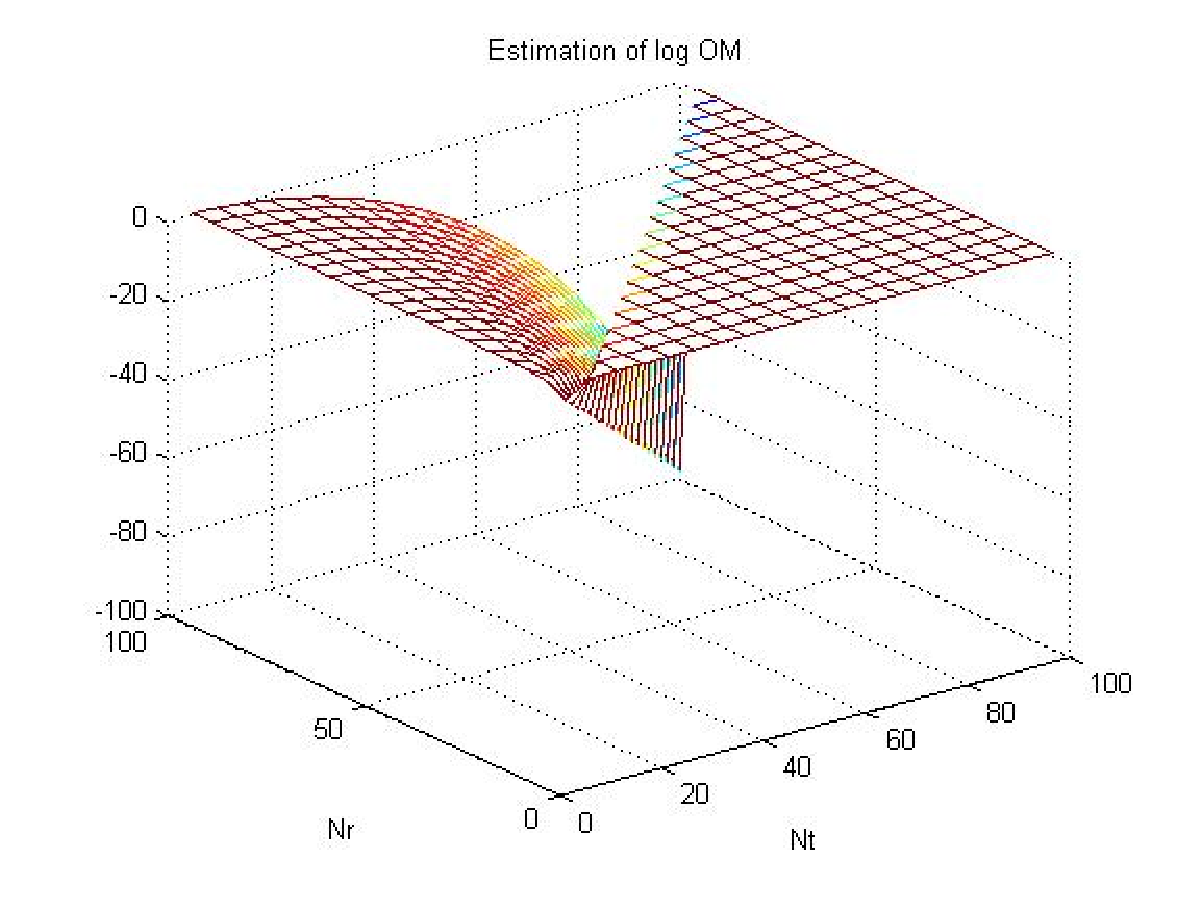
\includegraphics[width=0.7\textwidth, height=5cm]{logE_om_em.eps}
%\caption{Empirical Estimation $E[\ln(\phi_{om})]_{em}$}
%\label{figure1}
%\end{figure}

%\begin{figure}[htb]
%\centering
%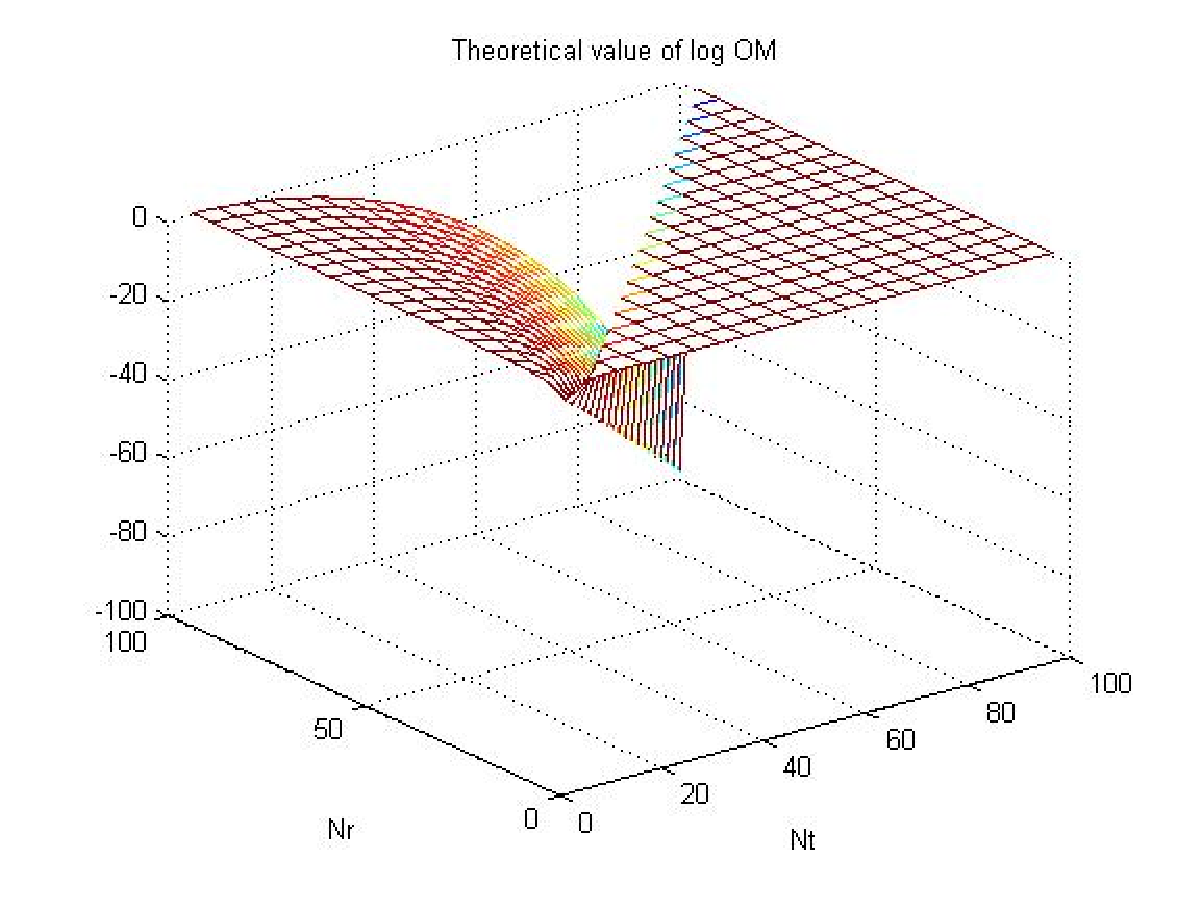
\includegraphics[width=0.7\textwidth, height=5cm]{logE_om_t.eps}
%\caption{Theoretical $E[\ln(\phi_{om})]_{t}$}
%\label{figure2}
%\end{figure} 


%\begin{figure}[htb]
%\centering
%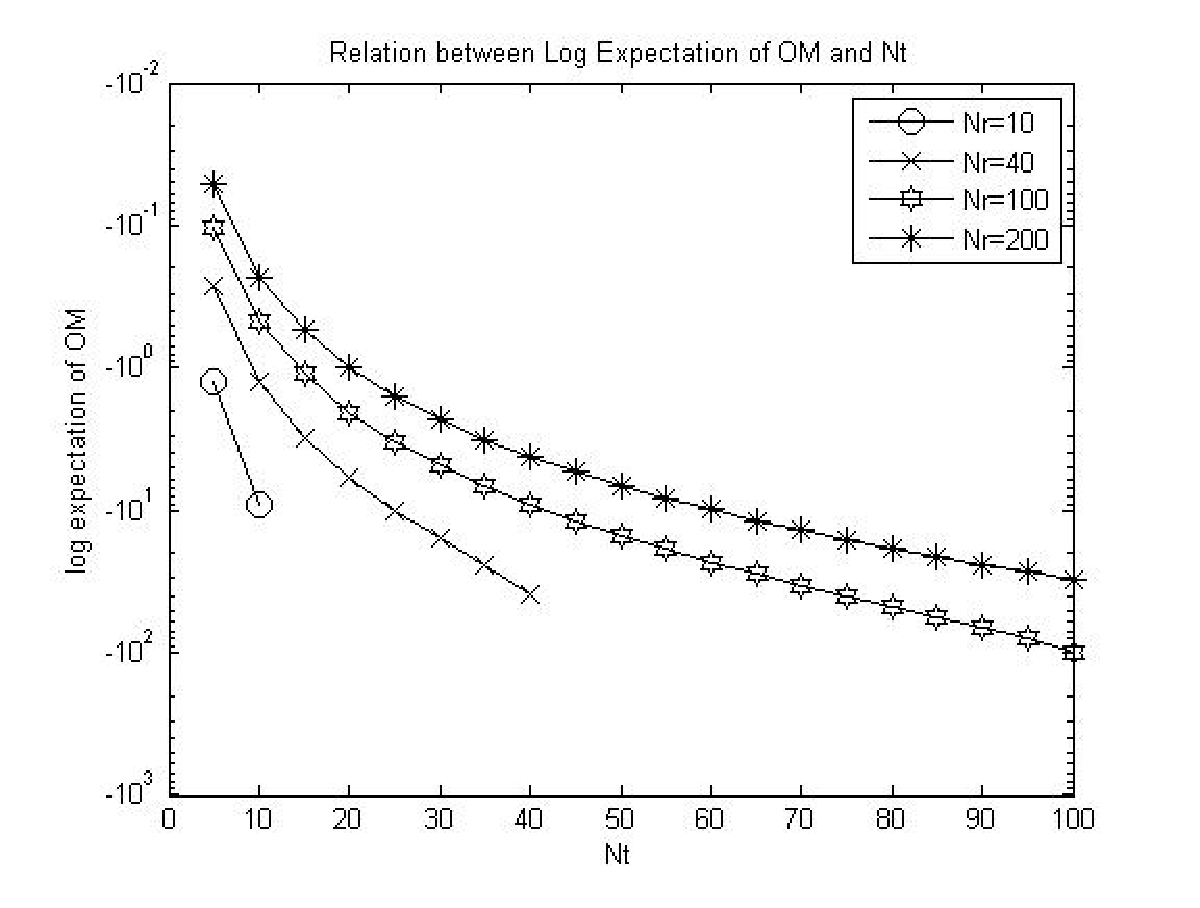
\includegraphics[scale=0.6]{NtE.eps}
%\caption{Relation between $N_{t}$ and $E[\ln(\phi_{om})]_{t}$}
%\label{figure3}
%\end{figure}


\section{Stopping Criteria}\label{stopping criteria}
As we have explained in section \ref{section lagrange duality}, the upper bound of Lagrangian dual objective function is determined by primal objective function, further more the optimal of primal and dual objective function is found if and only if the equality holds, that is 
\begin{equation}
\theta(\lambda^{r}, \lambda^{i})=f(\mathbf{w},\xi)
\label{duality equal}
\end{equation}
\begin{equation}
\frac{1}{2}||\mathbf{w}||^{2}_{\mathbb{H}}+C\sum_{i=1}^{N_{r}}[R(\xi^{r}_{i})+R(\hat{\xi}^{r}_{i})+R(\xi^{i}_{i})+R(\hat{\xi}^{i}_{i})],
\label{simple primal}
\end{equation}
(\ref{final complex lagrange duality}) can be rewritten as follow by substituting $\lambda^{r}=\alpha-\hat{\alpha}$, $|\lambda^{r}|=\alpha+\hat{\alpha}$ and $\lambda^{i}=\beta-\hat{\beta}$, $|\lambda^{i}|=\beta+\hat{\beta}$
\begin{IEEEeqnarray}[\relax]{l}
\nonumber
\theta(\lambda^{r}, \lambda^{i})=-\frac{1}{2}<(\lambda^{r})^{T}, \mathbf{K}^{r}\lambda^{r}>-\frac{1}{2}<(\lambda^{i})^{T}, \mathbf{K}^{r}\lambda^{i}>+<Re(\mathbf{y})^{T}, \lambda^{r}>+<Im(\mathbf{y})^{T}, \lambda^{i}>\\
-\epsilon<\mathbf{e}^{T}, (|\lambda^{r}|+|\lambda^{i}|)>+C\sum_{i=1}^{N_{r}}[\tilde{R}(\xi^{r}_{i})+\tilde{R}(\hat{\xi}^{r}_{i})+\tilde{R}(\xi^{i}_{i})+\tilde{R}(\hat{\xi}^{i}_{i})],
\label{simple dual function}
\end{IEEEeqnarray}
Similarly, (\ref{complex duality regularization1}) can be formulated as 
\begin{IEEEeqnarray}[\relax]{l}
||\mathbf{W}||^{2}_{\mathbb{H}}=<(\lambda^{r})^{T}, \mathbf{K}^{r}\lambda^{r}>+<(\lambda^{i})^{T}, \mathbf{K}^{r}\lambda^{i}>-2<\lambda^{r}, \mathbf{K}^{i}\lambda^{i}>,
\label{simple regularization}
\end{IEEEeqnarray}
hence, duality gap can be formulated as
\begin{IEEEeqnarray}[\relax]{l}
\nonumber
G(\lambda^{r}, \lambda^{i})=f(\mathbf{w},\xi)-\theta(\lambda^{r},\lambda^{i})=<(\lambda^{r})^{T}, \mathbf{K}^{r}\lambda^{r}>+<(\lambda^{i})^{T}, \mathbf{K}^{r}\lambda^{i}>-<Re(\mathbf{y})^{T}, \lambda^{r}>-<Im(\mathbf{y})^{T}, \lambda^{i}>\\
-\epsilon<\mathbf{e}^{T}, (|\lambda^{r}|+|\lambda^{i}|)>+C\sum_{i=1}^{N_{r}}[\xi^{r}_{i}R^{'}(\xi^{r}_{i})+\hat{\xi}^{r}_{i}R^{'}(\hat{\xi}^{r}_{i})+\xi^{i}_{i}R^{'}(\xi^{i}_{i})+\hat{\xi}^{i}_{i}R^{'}(\hat{\xi}^{i}_{i})]-2<\lambda^{r}, \mathbf{K}^{i}\lambda^{i}>.
\label{simple duality gap}
\end{IEEEeqnarray}
As we explained in section \ref{risk functional}, the choice of risk function is determined by distribution of noise, as to Gaussian noise, the risk function is 
\begin{equation}
R(\xi)=\frac{1}{2}\xi^{2},
\label{risk function1}
\end{equation} 
hence 
\begin{equation}
\tilde{R}(\xi)=R(\xi)-\xi R{'}(\xi)=-\frac{1}{2}\xi^{2},
\label{risk function2}
\end{equation}
In $\epsilon$-SVR, the objective to employ slack variables $\xi$ is to deal with the outliers that outside $\epsilon$ tube to compensate the influence from noise.
Therefore 
\begin{IEEEeqnarray}[\relax]{l}
\xi^{r}_{i}=Re(\mathbf{y}_{i})-Re(<\mathbf{h}_{i},\mathbf{w}>_{\mathbb{H}})-\epsilon\\
\hat{\xi}^{r}_{i}=Re(<\mathbf{h}_{i},\mathbf{w}>_{\mathbb{H}})-Re(\mathbf{y}_{i})-\epsilon
\label{outlier1}
\end{IEEEeqnarray}
Because $\xi^{r}\hat{\xi}^{r}=0$ (estimation can only exceed $\epsilon$ tube in one direction), therefore there is only one of $\xi$ and $\hat{\xi}$ need to be considered, thus 
\begin{IEEEeqnarray}[\relax]{l}
\xi^{r}_{i}(\hat{\xi}^{r}_{i})=\max(0, |Re(\mathbf{y}_{i})-Re(<\mathbf{h}_{i}, \mathbf{w}>_{\mathbb{H}})|-\epsilon)\\
\xi^{i}_{i}(\hat{\xi}^{i}_{i})=\max(0, |Im(\mathbf{y}_{i})-Im(<\mathbf{h}_{i}, \mathbf{w}>_{\mathbb{H}})|-\epsilon)\\
\xi\hat{\xi}=0,
\label{outlier2}
\end{IEEEeqnarray} 
Therefore the risk function can be rewritten as 
\begin{IEEEeqnarray}[\relax]{l}
R(\xi_{i}^{r})+R(\hat{\xi}_{i}^{r})=\frac{1}{2}(|Re(\mathbf{y}_{i})-Re(<\mathbf{h}_{i}, \mathbf{w}>_{\mathbb{H}})|)^{2}_{\epsilon}\\
\label{simple risk function1}
R(\xi_{i}^{i})+R(\hat{\xi}_{i}^{i})=\frac{1}{2}(|Im(\mathbf{y}_{i})-Im(<\mathbf{h}_{i}, \mathbf{w}>_{\mathbb{H}})|)^{2}_{\epsilon}
\label{simple risk function2}
\end{IEEEeqnarray}
where $()_{\epsilon}$ denotes $\epsilon$ insensitive function as we mention in section \ref{risk functional}. Based on (\ref{complex duality regression function}), we have 
\begin{IEEEeqnarray}[\relax]{l}
Re(\mathbf{y}_{i})-Re(<\mathbf{h}_{i}, \mathbf{W}>_{\mathbb{H}})=Re(\mathbf{y}_{i})-\sum_{j=1}^{N_{r}}\lambda^{r}_{j}\mathbf{K}^{r}_{ij}+\sum_{j=1}^{N_{r}}\lambda^{i}_{j}\mathbf{K}^{i}_{ij}\\
Im(\mathbf{y}_{i})-Im(<\mathbf{h}_{i}, \mathbf{W}>_{\mathbb{H}})=Im(\mathbf{y}_{i})-\sum_{j=1}^{N_{r}}\lambda^{i}_{j}\mathbf{K}^{r}_{ij}-\sum_{j=1}^{N_{r}}\lambda^{r}_{j}\mathbf{K}^{i}_{ij}
\label{intermediate function1}
\end{IEEEeqnarray}
we define two intermediate variables $\Phi$ and $\Psi$
\begin{IEEEeqnarray}[\relax]{l}
\label{intermedia function 2a}
\Phi^{r}=Re(\mathbf{y})-\mathbf{K}^{r}
\lambda^{r};
\Phi^{i}=Im(\mathbf{y})-\mathbf{K}^{r}\lambda^{i}\\
\Psi^{r}=\mathbf{K}^{i}\lambda^{i};
\Psi^{i}=-\mathbf{K}^{i}\lambda^{r}\\\label{intermediate function 2b}
\nonumber
\end{IEEEeqnarray} 
Therefore based on (\ref{simple risk function1})-(\ref{intermediate function2}), duality gap in (\ref{simple duality gap}) can be rewritten as 
\begin{IEEEeqnarray}[\relax]{l}
\nonumber
G(\lambda^{r}, \lambda^{i})=<(\lambda^{r})^{T}, \mathbf{K}^{r}\lambda^{r}>+<(\lambda^{i})^{T}, \mathbf{K}^{r}\lambda^{i}>-<Re(\mathbf{y})^{T}, \lambda^{r}>-<Im(\mathbf{y})^{T}, \lambda^{i}>\\
+\epsilon<\mathbf{e}^{T}, (|\lambda^{r}|+|\lambda^{i}|)>+C\sum_{i=1}^{N_{r}}[(|\Phi^{r}_{i}+\Psi^{r}_{i}|)^{2}_{\epsilon}+(|\Phi^{i}_{i}+\Psi^{i}_{i}|)^{2}_{\epsilon}]-2<\lambda^{r}, \mathbf{K}^{i}\lambda^{i}>.
\label{simple duality gap final}
\end{IEEEeqnarray}
Based on objective function in (\ref{simple dual function}), (\ref{simple duality gap final}) can be rewritten as 
\begin{IEEEeqnarray}[\relax]{l}
\nonumber
G=(\lambda_{r}, \lambda_{i})=<Re(\mathbf{y})^{T}, \lambda^{r}>+<Im(\mathbf{y})^{T}, \lambda^{i}>-\epsilon<\mathbf{e}^{T}, (|\lambda^{r}|+|\lambda^{i}|)>-2\theta(\lambda_{i}, \lambda_{j})\\
-2<\lambda^{r}, \mathbf{K}^{i}\lambda^{i}>.\label{simple duality gap ratio1}
\end{IEEEeqnarray}
The duality gap between primal problem and dual problem is used to evaluate how close a solution is to global minimum. In our scenario, duality gap is employed as stopping criteria.
Therefore to make stopping criteria more effective to monitor if algorithm convergent, we monitor the ratio by a value of tolerance (usually this tolerance is set to $10^{-3}$).
\begin{equation}
\frac{G}{G+\theta}
\label{simple duality gap ratio2}
\end{equation}
\subsection{Update $\Phi$, $\Psi$ and $G$}
Here we give the pseudo code to update $\Phi$, $\Psi$ and $G$.

Based on the definition of $\Phi$ and $\Psi$ in (\ref{intermedia function 2a}) and (\ref{intermediate function 2b}), we have the following procedure to update $\Phi$ and $\Psi$ in real channel and imaginary channel, assume the optimization coordinate updated in each channel are $1$ and $2$.\\
\begin{algorithm}[htb]
\begin{algorithmic}
\Procedure{\textbf{1}. Update $\Phi^{r}$ and $\Psi^{i}$ in real channel}{}
\For{$i=1:N_{r}$}
\State $\Phi_{i}^{r}=\Phi_{i}^{r}-\sigma_{1}^{r}\mathbf{K}^{r}_{i1}-\sigma_{2}^{r}\mathbf{K}_{i2}^{r}$
\State $\Psi_{i}^{i}=\Psi_{i}^{i}-\sigma_{1}^{r}\mathbf{K}^{i}_{i1}-\sigma_{2}^{r}\mathbf{K}^{i}_{i2}$
\EndFor
\EndProcedure
\end{algorithmic}
\end{algorithm}
\begin{algorithm}[htb]
\begin{algorithmic}
\Procedure{\textbf{2}. Update $\Phi^{i}$ and $\Psi^{r}$ in imaginary channel}{}
\For{$i=1:N_{r}$}
\State $\Phi_{i}^{i}=\Phi_{i}^{i}-\sigma_{1}^{i}\mathbf{K}^{r}_{i1}-\sigma_{2}^{i}\mathbf{K}_{i2}^{r}$
\State $\Psi_{i}^{r}=\Psi_{i}^{r}+\sigma_{1}^{i}\mathbf{K}^{i}_{i1}+\sigma_{2}^{i}\mathbf{K}^{i}_{i2}$
\EndFor
\EndProcedure
\end{algorithmic}
\end{algorithm}

Then the risk function term in (\ref{simple duality gap final}) is updated as following
\begin{algorithm}[htb]
\begin{algorithmic}
\Procedure{\textbf{3}. Update risk function in real channel}{$\chi^{r}$}
\State $\chi^{r}=0$  \Comment{initial risk term}
\For{$i=1:N_{r}$}
\If{$|\Phi^{r}_{i}+\Psi^{r}_{i}|>\epsilon$}
\State $\chi^{r}+=(|\Phi^{r}_{i}+\Psi^{r}_{i}|-\epsilon)^{2}$
\EndIf
\EndFor
\EndProcedure
\end{algorithmic}
\end{algorithm}

\begin{algorithm}[htb]
\begin{algorithmic}
\Procedure{\textbf{4}. Update risk function in imaginary channel}{$\chi^{i}$}
\State $\chi^{i}=0$  \Comment{initial risk term}
\For{$i=1:N_{r}$}
\If{$|\Phi^{i}_{i}+\Psi^{i}_{i}|>\epsilon$}
\State $\chi^{i}+=(|\Phi^{i}_{i}+\Psi^{i}_{i}|-\epsilon)^{2}$
\EndIf
\EndFor
\EndProcedure
\end{algorithmic}
\end{algorithm}
The pseudo code to update duality gap $G$ based on (\ref{simple duality gap final}) is shown as follow (assume the coordinate updated in real channel is $i$ and $j$, in imaginary channel is $m$ and $f$.
\begin{algorithm}[htb]
\begin{algorithmic}
\Procedure{\textbf{5}. Update $G$}{ratio of $G$}
\State $G+=Re(\mathbf{y}_{1})\sigma^{r}_{i}+Re(\mathbf{y}_{2})\sigma^{r}_{j}$
\State $G+=Im(\mathbf{y}_{1})\sigma^{i}_{m}+Re(\mathbf{y}_{2})\sigma^{i}_{f}$
\State $G-=\epsilon(|\lambda^{r}_{i}+\sigma^{r}_{i}|-|\lambda^{r}_{i}|+|\lambda^{r}_{j}+\sigma^{r}_{j}|-|\lambda^{r}_{j}|)$
\State $G-=\epsilon(|\lambda^{i}_{m}+\sigma^{i}_{m}|-|\lambda^{i}_{m}|+|\lambda^{i}_{f}+\sigma^{i}_{f}|-|\lambda^{i}_{f}|)$
\State $G-=2(\bigtriangledown \theta(\sigma^{r}_{i},\sigma^{r}_{j},\sigma^{i}_{m},\sigma^{i}_{f}))$
\State $G-=$
\EndProcedure
\label{update G Phi and Psi}
\end{algorithmic}
\end{algorithm}


Here we give the pseudo code for sequential 1-D searching 2-D solver

\begin{algorithm}[htb]
\begin{algorithmic}
\Procedure{CSVD}{$\mathbf{y}$,$\mathbf{H}$}
\State Step 1. Initialization
\For{$i=1:N_{r}$}\Comment{initialize $\lambda^{r}$, $\lambda^{i}$, $\Phi^{r}$, $\Phi^{i}$, $\Psi^{r}$, $\Psi^{i}$ and duality gap $G$}
\State $\lambda_{i}^{r}=0, \lambda_{i}^{i}=0$
\State $\Phi_{i}^{r}=Re(y_{i}), \Phi_{i}^{i}=Im(y_{i})$
\State $\Psi_{i}^{r}=0, \Psi_{i}^{i}=0$
\EndFor 
\State  Step 2. if $G>tol$, go to step 3, else go to Step 6
\State Step 3.
\State Sequentia 1-D searching 2-D solver with or without damping \Comment{find two optimization variables to be updated} 
\State Step 4.
\State \textbf{Procedure 1} update $G$, $\Phi$ and $\Psi$
\State Step 5.
\State $\tilde{x}=(\lambda^{r}+i\lambda^{i})\mathbf{H}$ \Comment{reconstruct $\mathbf{x}$}
\State $\mathbf{x}=\mathbb{Q}(\tilde{x})$\Comment{$\mathbb{Q}(\cdot)$ denotes quantization operation based on symbol constellation}
\State go back to Step 2
\State Step 6. \textbf{Return} $\mathbf{x}$ 

\EndProcedure
\end{algorithmic}
\label{CSVD algorithm}
\caption{Dual Channel Complex Support Vector Detection Algorithm }
\end{algorithm}

\begin{algorithm}[htb]
\begin{algorithmic}
\Procedure{\textbf{2}. Sequential 2-D solver without Damping}{$1st$, $2nd$} 
\For{$i=1:N_{r}$}
\State update $\lambda^{r}_{i}(\lambda_{i}^{i})$ by single direction solver
\State calculate $\bigtriangledown \theta^{r}_{i}(\bigtriangledown \theta_{i}^{i})$\Comment{ calculate the gain of sub objective function}
\EndFor
\State choose the dual variable with first and the second largest gain of sub objective function, denoted as 1st and 2nd
\State update $\Phi^{r}(\Phi^{i})$ and $\Psi^{r}(\Psi^{i})$ with respect to 1st and 2nd
\State \textbf{Return} 1st, 2nd
\EndProcedure
\end{algorithmic}
%\caption{Sequential 2-D Solver without Damping}
\label{1D2D Nodamping}
\end{algorithm} 
 
 
 \begin{algorithm}
\begin{algorithmic}
\Procedure{\textbf{3}. Sequential 2-D solver with Damping}{$1s_{1}t$,$1st_{2}$}
\For{$i=1:N_{r}$}\Comment{First round searching}
\State update $\lambda_{i}^{r}(\lambda_{i}^{i})$ by single direction solver
\State calculate $\bigtriangledown \theta_{i}^{r}(\bigtriangledown \theta_{i}^{i})$ \Comment{calculate the gain of objective function}
\EndFor
\State choose the dual variable with the largest gain of objective function as $1st_{1}$
\State update $\Phi^{r}(\Phi^{i})$ and $\Psi^{r}(\Psi^{i})$ with respect to $1st_{1}$
\For{$i=1:N_{r}$} \Comment{Second round searching}
\State update $\lambda_{i}^{r}(\lambda_{i}^{i})$ by single direction solver
\State calculate $\bigtriangledown \theta_{i}^{r}(\bigtriangledown \theta_{i}^{i})$ \Comment{calculate the gain of objective function}
\EndFor
\State choose the dual variable with the largest gain of objective function as $1st_{2}$
\State update $\Phi^{r}(\Phi^{i})$ and $\Psi^{r}(\Psi^{i})$ with respect to $1st_{2}$
\State \textbf{Return} $1st_{1}$ and $1st_{2}$
\EndProcedure
\end{algorithmic}
%\caption{Sequential 2-D Solver with Damping}
\label{1D2D damping}
\end{algorithm} 
 
\section{Hyperparameter Setting}

\section{Computer Simulations}
Computer simulation is launched to test the detection and run time performance of proposed dual channel complex support vector detection algorithm. For sake of brevity, the real case is tested first, all the experiments are made by C, compiled by gcc version 4.8.3 on 64 bit Fedora (release 19) Linux system. The experiment platform is a desktop computer with I5-4th generation CPU with quad processing cores, 3.2 GHz clock rate, 8 GB RAM. 

For sake of brevity, we consider a real uncoded spatial multiplex large MIMO system to simulate one channel of the proposed dual channel complex support vector detection algorithm.  with $N_{r}$ received antennas and $N_{t}$ transmitted antennas. The propagation channel matrix is constructed by channel gain components that are identically independent distributed (i.i.d) Gaussian random variables with zero mean and unit variance. transmitted symbols are mutually independent modulated by $M$ PAM with normalized average energy $\frac{1}{N_{t}}$, transmitted over flat fading channel, the sample of noise is AWGN with zero mean and variance $\frac{1}{10^{SNR/10}}$, where $SNR$ denotes the signal to noise ratio. 
We make experiment to low loading factor system $100\times 40$ and full loading factor $100\times 100$, Fig \ref{SER performance} shows the symbol error rate (SER) performance.  
\begin{figure}
\centering
\def\svgwidth{\columnwidth}
\input{BER_curve_real_system.pdf_tex}
\caption{SER performance of $100\times 100 $ and $100\times 40$ MIMO system}
\label{SER performance}
\end{figure}
% An example of a floating figure using the graphicx package.
% Note that \label must occur AFTER (or within) \caption.
% For figures, \caption should occur after the \includegraphics.
% Note that IEEEtran v1.7 and later has special internal code that
% is designed to preserve the operation of \label within \caption
% even when the captionsoff option is in effect. However, because
% of issues like this, it may be the safest practice to put all your
% \label just after \caption rather than within \caption{}.
%
% Reminder: the "draftcls" or "draftclsnofoot", not "draft", class
% option should be used if it is desired that the figures are to be
% displayed while in draft mode.
%
%\begin{figure}[!t]
%\centering
%\includegraphics[width=2.5in]{myfigure}
% where an .eps filename suffix will be assumed under latex, 
% and a .pdf suffix will be assumed for pdflatex; or what has been declared
% via \DeclareGraphicsExtensions.
%\caption{Simulation results for the network.}
%\label{fig_sim}
%\end{figure}

% Note that IEEE typically puts floats only at the top, even when this
% results in a large percentage of a column being occupied by floats.


% An example of a double column floating figure using two subfigures.
% (The subfig.sty package must be loaded for this to work.)
% The subfigure \label commands are set within each subfloat command,
% and the \label for the overall figure must come after \caption.
% \hfil is used as a separator to get equal spacing.
% Watch out that the combined width of all the subfigures on a 
% line do not exceed the text width or a line break will occur.
%
%\begin{figure*}[!t]
%\centering
%\subfloat[Case I]{\includegraphics[width=2.5in]{box}%
%\label{fig_first_case}}
%\hfil
%\subfloat[Case II]{\includegraphics[width=2.5in]{box}%
%\label{fig_second_case}}
%\caption{Simulation results for the network.}
%\label{fig_sim}
%\end{figure*}
%
% Note that often IEEE papers with subfigures do not employ subfigure
% captions (using the optional argument to \subfloat[]), but instead will
% reference/describe all of them (a), (b), etc., within the main caption.
% Be aware that for subfig.sty to generate the (a), (b), etc., subfigure
% labels, the optional argument to \subfloat must be present. If a
% subcaption is not desired, just leave its contents blank,
% e.g., \subfloat[].


% An example of a floating table. Note that, for IEEE style tables, the
% \caption command should come BEFORE the table and, given that table
% captions serve much like titles, are usually capitalized except for words
% such as a, an, and, as, at, but, by, for, in, nor, of, on, or, the, to
% and up, which are usually not capitalized unless they are the first or
% last word of the caption. Table text will default to \footnotesize as
% IEEE normally uses this smaller font for tables.
% The \label must come after \caption as always.
%
%\begin{table}[!t]
%% increase table row spacing, adjust to taste
%\renewcommand{\arraystretch}{1.3}
% if using array.sty, it might be a good idea to tweak the value of
% \extrarowheight as needed to properly center the text within the cells
%\caption{An Example of a Table}
%\label{table_example}
%\centering
%% Some packages, such as MDW tools, offer better commands for making tables
%% than the plain LaTeX2e tabular which is used here.
%\begin{tabular}{|c||c|}
%\hline
%One & Two\\
%\hline
%Three & Four\\
%\hline
%\end{tabular}
%\end{table}


% Note that the IEEE does not put floats in the very first column
% - or typically anywhere on the first page for that matter. Also,
% in-text middle ("here") positioning is typically not used, but it
% is allowed and encouraged for Computer Society conferences (but
% not Computer Society journals). Most IEEE journals/conferences use
% top floats exclusively. 
% Note that, LaTeX2e, unlike IEEE journals/conferences, places
% footnotes above bottom floats. This can be corrected via the
% \fnbelowfloat command of the stfloats package.
\section{Complexity Analysis}


\section{Conclusion}
The conclusion goes here.





% if have a single appendix:
%\appendix[Proof of the Zonklar Equations]
% or
%\appendix  % for no appendix heading
% do not use \section anymore after \appendix, only \section*
% is possibly needed

% use appendices with more than one appendix
% then use \section to start each appendix
% you must declare a \section before using any
% \subsection or using \label (\appendices by itself
% starts a section numbered zero.)
%


\appendices
%\section{Proof of the First Zonklar Equation}
Appendix one text goes here.

% you can choose not to have a title for an appendix
% if you want by leaving the argument blank
\section{}
Appendix two text goes here.


% use section* for acknowledgment
%\section*{Acknowledgment}


%The authors would like to thank...


% Can use something like this to put references on a page
% by themselves when using endfloat and the captionsoff option.
\ifCLASSOPTIONcaptionsoff
  \newpage
\fi



% trigger a \newpage just before the given reference
% number - used to balance the columns on the last page
% adjust value as needed - may need to be readjusted if
% the document is modified later
%\IEEEtriggeratref{8}
% The "triggered" command can be changed if desired:
%\IEEEtriggercmd{\enlargethispage{-5in}}

% references section

% can use a bibliography generated by BibTeX as a .bbl file
% BibTeX documentation can be easily obtained at:
% http://www.ctan.org/tex-archive/biblio/bibtex/contrib/doc/
% The IEEEtran BibTeX style support page is at:
% http://www.michaelshell.org/tex/ieeetran/bibtex/
%\bibliographystyle{IEEEtran}
% argument is your BibTeX string definitions and bibliography database(s)
%\bibliography{IEEEabrv,../bib/paper}
%
% <OR> manually copy in the resultant .bbl file
% set second argument of \begin to the number of references
% (used to reserve space for the reference number labels box)
%\begin{thebibliography}{1}

%\bibitem{IEEEhowto:kopka}
%H.~Kopka and P.~W. Daly, \emph{A Guide to \LaTeX}, 3rd~ed.\hskip 1em plus
%  0.5em minus 0.4em\relax Harlow, England: Addison-Wesley, 1999.

%\end{thebibliography}

% biography section
% 
% If you have an EPS/PDF photo (graphicx package needed) extra braces are
% needed around the contents of the optional argument to biography to prevent
% the LaTeX parser from getting confused when it sees the complicated
% \includegraphics command within an optional argument. (You could create
% your own custom macro containing the \includegraphics command to make things
% simpler here.)
%\begin{IEEEbiography}[{\includegraphics[width=1in,height=1.25in,clip,keepaspectratio]{mshell}}]{Michael Shell}
% or if you just want to reserve a space for a photo:

%\begin{IEEEbiography}{Michael Shell}
%Biography text here.
%\end{IEEEbiography}

% if you will not have a photo at all:
%\begin{IEEEbiographynophoto}{John Doe}
%Biography text here.
%\end{IEEEbiographynophoto}

% insert where needed to balance the two columns on the last page with
% biographies
%\newpage

%\begin{IEEEbiographynophoto}{Jane Doe}
%Biography text here.
%\end{IEEEbiographynophoto}

% You can push biographies down or up by placing
% a \vfill before or after them. The appropriate
% use of \vfill depends on what kind of text is
% on the last page and whether or not the columns
% are being equalized.

%\vfill

% Can be used to pull up biographies so that the bottom of the last one
% is flush with the other column.
%\enlargethispage{-5in}



% that's all folks
%\end{spacing}

\newpage
\bibliographystyle{IEEEtran}
\bibliography{citation}	
\end{spacing}												
\end{document}




